\chapter{Detectors}\label{chap:detectors}

The detector packages of the SHMS and HMS must perform at least two
functions: tracking and
particle identification (PID).
A particle traversing the detector stack
encounters two sets of drift chambers with six planes of sense
wires in each chamber. From the chamber information both positions
and angles in the dispersive and transverse directions can be determined.
The information from these chambers is the principal input
of the tracking algorithms.

% Some details have to be changed to encompase differences in SHMS
The chambers are followed by two planes of hodoscopes designated S1X and S1Y.
These plastic scintillator arrays provide the timing reference for the
drift chambers, are used in trigger formation, and in combination
with a second hodoscope pair, provide time-of-flight particle identification.
These scintillators can also be used to perform crude tracking.

The next element encountered by a particle is a gas threshold Cerenkov detector.
This is used for particle identification. In the SOS spectrometer, this
gas threshold Cerenkov detector can be replaced by an Aerogel detector,
with a similar function.

The second hodoscope pair, S2X and S2Y, is located directly behind the
gas Cerenkov. Their function is essentially the same as that of S1X and S1Y.
In the SOS spectrometer, an option exists to have this hodoscope pair
be preceded by a third chamber to improve tracking.

The final element in the detector stack is the lead glass shower calorimeter.
This is used for energy determination and PID.


\section{Common Systems}
This section describes systems that are common to the detectors in both
spectrometers.

\subsection{CAEN High Voltage System}

\paragraph{Overview}

The CAEN Distributed High Voltage System is responsible for
providing high voltage power to all HMS and SOS detector systems
including phototubes for hodoscopes, Cerenkov detectors, and shower
counters as well as wire voltages for drift chambers.  This is in
general a networked system made up of individual crates (Controllers)
each of which can hold up to four independent high voltage modules
(Cards).  Each card provides 16 channels of high voltage output (SHV
connectors).  There are three flavors of Cards which are in use with the
Hall~C detector systems, they are listed in Table~\ref{tab:hv_cards}.  All types of Cards 
can in general be intermixed within a Crate.


\begin{table}
\caption{Specifications of High-Voltage Cards used in Hall~C Detector 
Systems\label{tab:hv_cards}.}
\begin{center}
\begin{tabular}{ccccc}
        &Card type      &Max Voltage    &Max Current    &Detector System \\
	&		&		&		&	\\
	& A403 (or A503)&--3000V		&3.0mA		&Hodo/Shower\\
	& A503P		&+3000V		&3.0mA		&Cerenkov\\
	& A505		&--3000V		&200$\mu$A 	&Drift Chambers\\
  \end{tabular}
\end{center}
\end{table}

The system can be controlled/monitored both locally (by a built-in
display panel on the individual Crates) or remotely by either a
connected Terminal (RS232) or VME CAEN net interface card (Model V288).


\begin{figure}
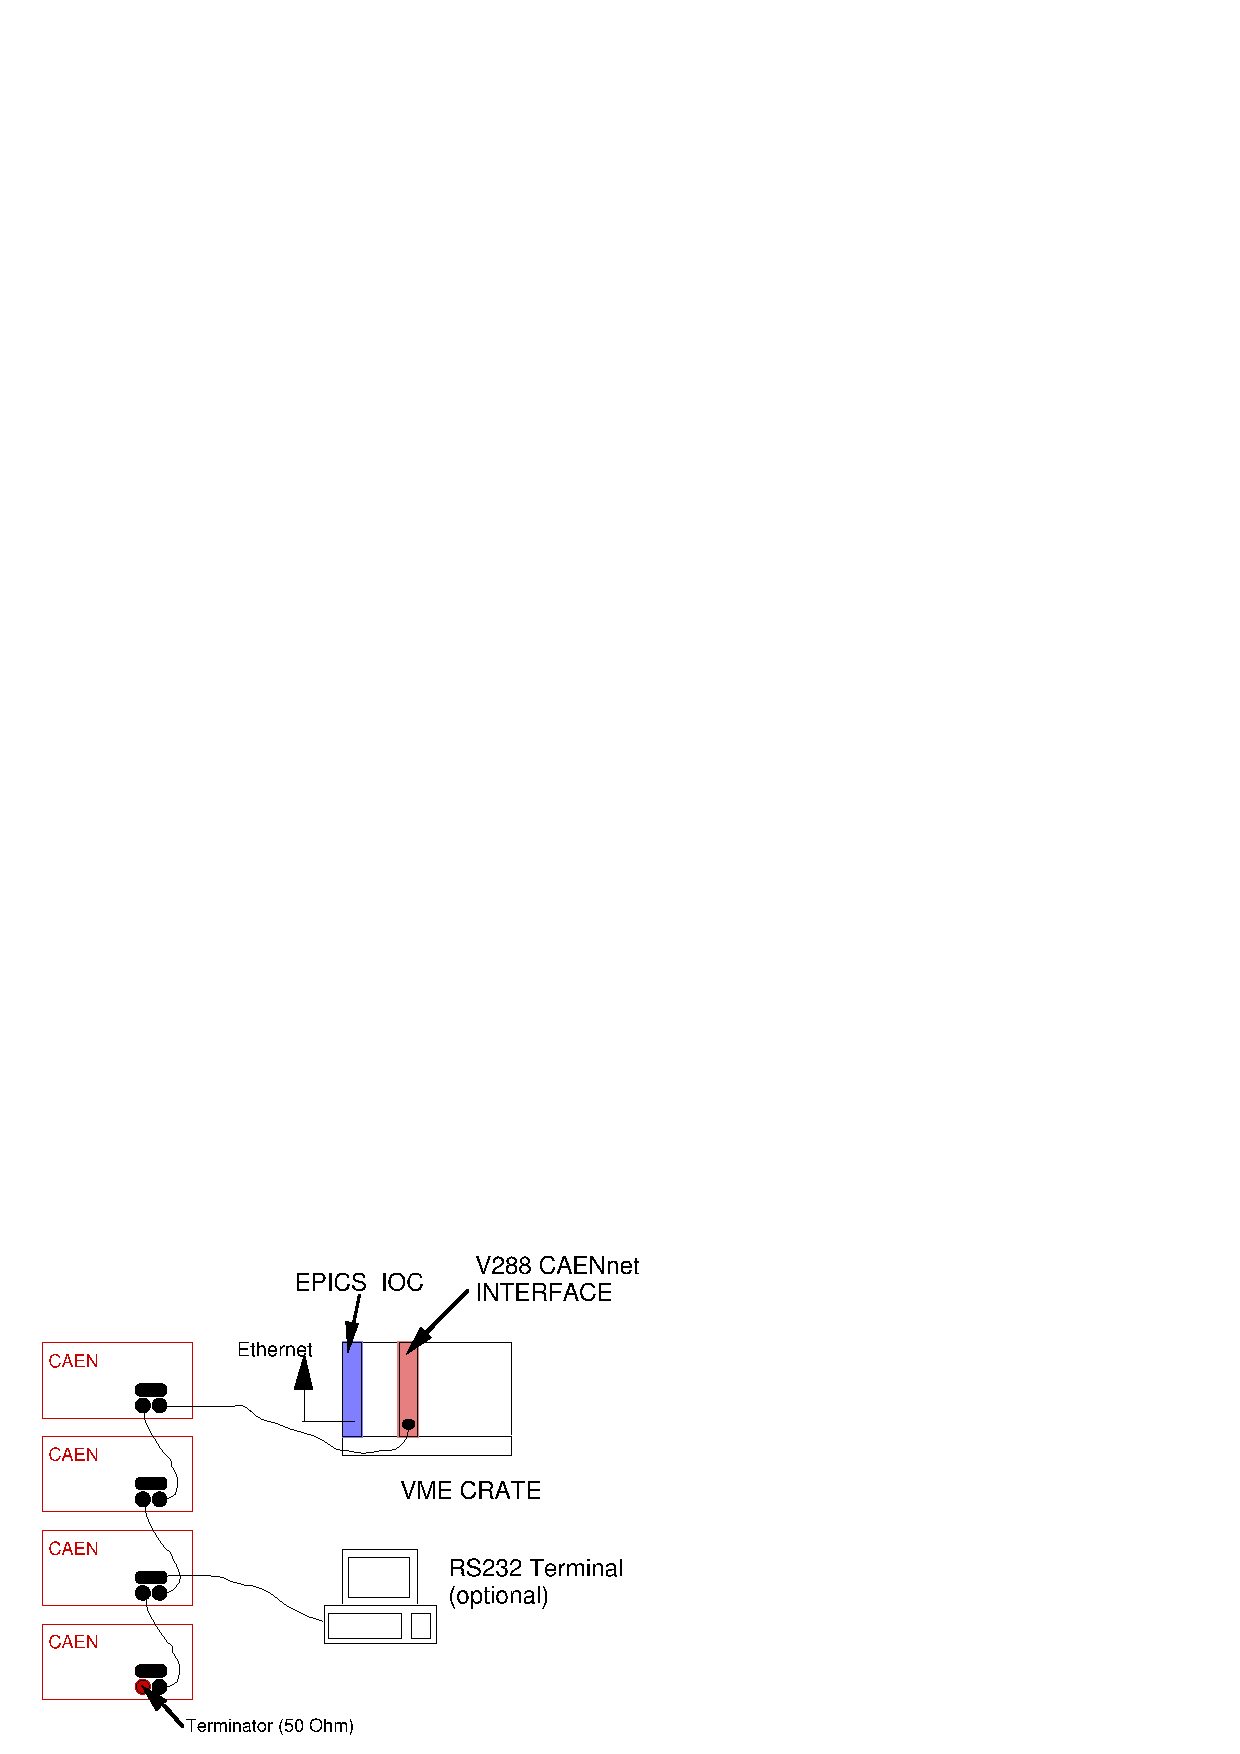
\includegraphics[height=4.5in]{CAENHV.pdf}
\caption{Generic CAEN High Voltage System setup\label{fig:caen_setup}}
\end{figure}

HV channel assignments currently in effect are indicated in 
two files ("group\_map" and
"channel\_map") in the directories \$EPHHV/perl (for HMS) and \$EPSHV/perl (for
SOS) when you are logged in as cvxwrks to one of the cdaq machines.

%\vfil\eject
\paragraph{General Operation}

\subparagraph{Normal Operation:}

In general the high voltage system will be controlled or monitored
from the counting house using the EPICS slow control system which will
be interfaced through a V288 card located in a VME crate in rack CH03B13
in the electronics room of the counting house
(see Figure~\ref{fig:caen_setup}).  It is also possible, but not recommended,
to control a CAEN crate using its front panel display or a terminal
if one is connected to the crate.
For EPICS control/monitoring all crates must be interconnected with 50
ohm (terminated) cable and all crates must be powered on whether they
will be in use or not.

Configuration of individual HV output channels is done through a
text file which is read in and downloaded when EPICS control is
configured. Step by step instructions for modifying this file and
reconfiguring the system are provided in the document
\htmladdnormallink{$\sim$cdaq/documents/slow\_controls/hvcntl.text}{http://www.jlab.org/Hall-C/document/slow_controls/hvcntl.text}. Do the HV rebuilds on cdaqs1 as cvxwrks.


It is imperative that
you follow the steps as shown there and not try to invent your own
procedure.
All relevant parameters
can be programmed through this interface.  The user must only know the
Crate Numbers and the Channel Numbers that his equipment is connected
to.  The crate number can be gotten from the front panel display and the
channel numbers run from 0-63 for each crate ( If only three cards are
installed, the channel number will run from 0-47 top to bottom
regardless of their positions in the crate).

\subparagraph{Important Features:}

The user can program several important features for individual
cards and/or channels.  The most common are:

\begin{itemize}
\item{HV limits -- 2 types including a hardware maximum (common to a
card) set with a pot on the front panel of each card and a software
maximum for each channel.}
\item{Current Trip Value -- The current over which the system will
indicate an alarm status and initiate a trip off of that channel.}
\item{Current Trip Time -- The amount of time the system will allow
the alarm condition before actually switching off that channel.}
\item{Ramp-up Value -- The number of volts/sec the voltage will ramp
to its set point upon switching on the channel.}
\item{Other Features -- See the CAEN Technical Information Manual.}
\end{itemize}

\subparagraph{Remote Operation: the High Voltage GUI system}
Remote operation of the CAEN system is described in the section
\ref{par:hv_ops}.

\subparagraph{Local (Front Panel) Operation}

Modifications to the parameter settings should in general not be
made at the front panel or through a locally connected terminal if the
EPICS system is in operation.  This mode of control is meant for
diagnostics and testing of a detector system prior to running.  There is
only one feature which must be set at the front panel before initiating
an EPICS control session - this is the crate number.  The RS232
parameters must also be set from the front panel ( suggested default are
9600 baud  no parity  1 stop bit).

If unfamiliar with the operation of the HV system in local modes
one should get experienced personnel or review the CAEN Technical
Information Manual.

\paragraph{Safety Concerns/Caveats}

There are a number of cautions one should observe when operating
the CAEN HV equipment to avoid damage and insure proper functioning:

\begin{itemize}
\item{Use only proper SHV connectors and approved cables when
connecting equipment to the supply.}
\item{{\bf DO NOT} attach/remove HV cables when loads are present on the
channel ( a red LED above each channel indicates the presence of a
load).}
\item{Insure adequate ventilation around crates to avoid overheating
of the electronics.}
\item{Wait 2-3 minutes after switching off a crate before removal of a
HV card.}
\item{Insure proper static precautions when handling HV cards.}
\end{itemize}

For proper EPICS control operation:

\begin{itemize}
\item{Inter-crate connections must be unbroken and terminated at the
last crate at 50 Ohms.  All crates must be powered on.}
\item{Crate numbers for each crate in the chain must be distinct and
different from 0 (i.e. 1-99)}
\item{The HV Enable switch (on the front panel of each crate) must be on.}
\item{One should refrain from any local operation of crates when the
EPICS system is active.}
\end{itemize}

\subsection{The Gas Mixing System}

The Hall~C On-line gas mixing system exists in the gas shed located
to the left of the counting house in the parking lot between the counting house
and the accelerator service building.
It provides two parallel
flow-controlled gas streams from a common source.  Flow rates, and gas mix
can be controlled independently in each of the gas streams.  The main
component of the system is a single MKS 647 menu driven 4-channel
controller that operates both of the parallel systems.  Gas flow is
controlled by 2259c proportional mass flow control valves.  The 647 allows
the Gas Calibration factor to be altered in software, allowing the user to
change to a different gas without recalibration of the mass flow control
valves.

A temperature controlled alcohol bubbler is provided for each gas
stream.  The alcohol level in each stream is maintained by a float valve
fed from a reservoir outside the bubbler chiller. This allows the alcohol
system to be refilled without opening the system to air.  A sight glass on
the side of the reservoir allows the level to be monitored.  A by-pass loop
around each alcohol system is provided should alcohol free gas be desired
or if the alcohol system requires maintenance.

The 647 is factory upgradeable to 8 channels.  The gas mixing
system has been plumbed to provide 2 parallel 3 channel gas streams.  In
the original installation, the mass flow control valves for channels 5 and
6 (gas \#3) were not installed.

To upgrade to 6 channel operation, 2 additional 2259c valves need
to purchased and installed.  The 647 needs to be returned to the factory
for the upgrade to 8 channel operation

The system will support a remote monitor and remote control through
a separate display port and an RS232 port on the back of the MKS 647 unit.

{\bf This system operates by measuring and controlling flow rate instead
of pressure. This system will maintain a constant rate of flow
regardless of pressure. It should not be used without appropriate pressure
relief device such as relief bubblers and relief valves. It should not be
connected to a closed vessel or system.}

{\bf Warning:} {\em{When using flow controlled systems such as this one, one 
must never introduce gas into a vessel without insuring that an outlet from the vessel is 
open.  The gas will continue to flow at the flow rate set point until the gas 
reaches the pressure setting of the pressure device ie. the regulator or relief 
bubbler, or until the vessel fails}.}

The manual valves used in this system are numbered on their
handles.  Those numbers are referenced in this document and in
Figure~\ref{fig:gas_mix}.
\begin{figure}
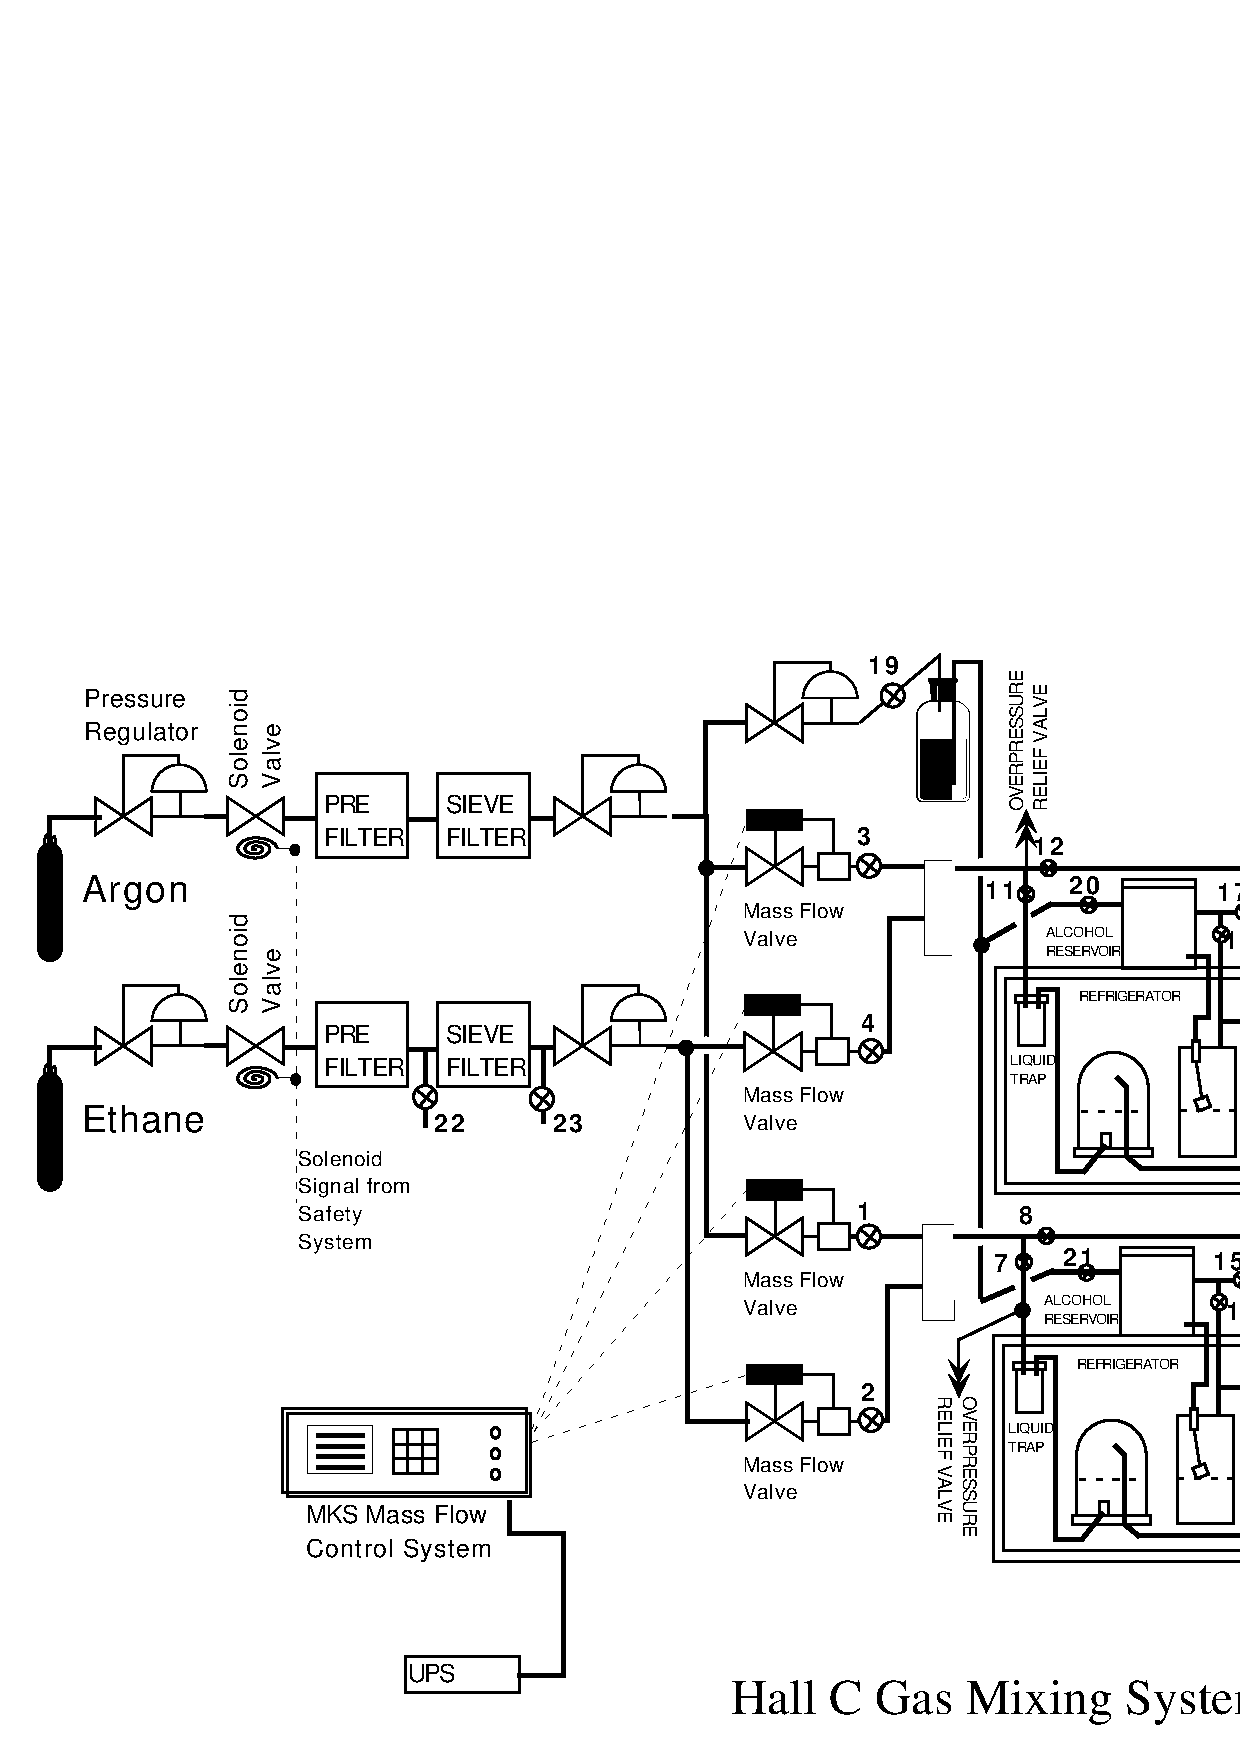
\includegraphics[width=6in,bb=12 12 750 590]{HallCGasMixlvl1.pdf}
\caption{Diagram of Hall~C Gas Mixing System\label{fig:gas_mix}}
\end{figure}

\paragraph{Normal Operation.}

For normal operation, with the alcohol systems in use, the following valves
should be set as follows:

{\bf For The HMS:}

Open - 3, 4, 11, 14; Closed - 12, 13, 17, 18, 19, 20


Unless the gas \#3 Mass flow control valve is installed, valve \#6 should
always be closed.

{\bf For the SOS:}

Open - 1, 2, 7, 10; Closed - 8, 9, 15, 16, 19, 21.


Unless the gas \#3 Mass flow  control valve is installed, valve \#5 should
always be closed.

\paragraph{Operating the MKS 647 Mass Flow Controller.}

The gas flow is controlled by a MKS 647 controller and mass flow
control valves.  The 647 is menu driven from a CRT in the front panel and
with a keypad with cursor controls. The 647 features a non-volatile memory
so settings are retained even if the unit is unpowered.  The initial menu
upon startup is the Command Menu.  For normal operation use either the User
Display menu (Command menu item \#1) or the Extended Display menu (Command
menu item \#2).  The User Display menu shows actual flow in each channel and
the total flow in all channels.  The Extended Display menu shows actual
flow, flow set point, units, valve full scale range, gas calibration
factor, whether that channel is enabled, and whether each channel is
operating in master, slave, or independent mode.

{\bf To set flow rates:}

The flow rate set points are adjusted from the Extended Display
menu.  There are two methods to change valve flow rate set point.  If you
want to enter a specific value you must first turn off the flow in that
channel or all of the channels.  Using the cursor keys move the cursor to
the desired channel.  Enter the desired flow rate.

The flow rate set point can be changed with gas flowing using the
cursor keys. In the Extended Display mode move the cursor to the desired
channel using the left/right cursor keys.  The set point can then be
adjusted up or down using the cursor up/down keys.

{\bf To turn gas flow on or off:}

The gas flow can be turned on or off while in any menu.  When any
of the mass flow valves are open the green LED labeled ``GAS ON" on the 647
is lit.  When none of the gas flow valves are open the red ``STAND BY" LED
will be flashing.  In the Extended Display menu the bottom line displays on
or off, by channel, to show which mass flow valves are enabled.  The green
LED must be lit and an ``ON" must be displayed in the bottom row of the
Extended Display menu for gas to be flowing in a particular channel.

{\bf Turning the gas on or off is done in two steps which can be done in
either order.}
Each channel must be enabled by pressing ``ON" and then
that channel number.  The command input must be enabled by pressing ``ON"
and then ``ALL" from the keypad.  This allows a single channel or all of the
enabled channels to be turned on or off at once.  Both steps must be
performed initially, but thereafter only one of the steps need be performed
to cycle the gas flow on or off.

To turn gas off in a single channel press ``OFF" and then the
desired channel.  If you want to close all the valves simultaneously, press
the ``OFF" key and then the ``ALL/0" key.  To turn gas back on you must
reverse whichever sequence you used to stop the gas flow.  For example if
you turned the gas off by pressing ``OFF" and then the channel number, it
must be turned back on by pressing ``on" and then the channel number.  If
you turn off all the channels by pressing ``OFF" , ``ALL" you must turn it
back on by pressing ``ON" , ``ALL."

{\bf To by-pass the alcohol system:}

For the HMS:
Open valves 12 \& 13, then close valves 11 \& 14, in that order!

For the SOS:
Open valves 8 \& 9, then close valves 7 \& 10, in that order!

{\bf To refill the alcohol bubblers:}

The alcohol bubbler system features a refill system that allows
filling directly from the bottle, minimizing exposure of the alcohol to air
and reducing the possibility of a spill.
{\bf The reservoirs should be refilled
before they become empty to maintain a head of liquid over the float valve
which will prevent air from entering the system.}
In the back of the gas
system rack is a holder for gallon sized alcohol bottles and a cap with dip
tube.  Place a new bottle in the bottle holder and replace the cap with the
cap with dip tube.

\begin{itemize}
\item{ \bf{Step-by-Step Instructions for Refilling the SOS Alcohol Bubbler}\\
\em{These steps must be individually completed in the order listed!}}\\
Refer to Fig.~\ref{fig:gas_mix}. 
\begin{enumerate}
\item{If needed, install a full bottle of alcohol in the back of the gas racks as mentioned in the preceeding paragraph.}
\item{{\em Open valves 8,9. Close valves 7,10} to Put the SOS alcohol bubbler in BYPASS.}
\item{{\em Close valve 16} to isolate the warm reservoir gas from the bubbler.}
\item{{\em Open valve 15} to bleed off the warm reservoir gas pressure.}
\item{{\em Open valve 19} to pressurize the alcohol bottle.}
\item{{\em Open valve 21} to flow alcohol into the warm reservoir.}
\item{When the alcohol level in the sight-glass is within 2cm of the top, stop
the flow of alcohol: {\em Close valve 21.}}
\item{{\em Close valve 19.}}
\item{{\em Open valve 16.}}
\item{{\em Close valve 15.}}
\item{{\em Open Valves 7 and 10. Close Valves 8 and 9.}}
\item{Record what you did in both the gas logbook and the electronic logbook.} 
\end{enumerate}

\item{ \bf{Step-by-Step Instructions for Refilling the HMS Alcohol Bubbler}\\
\em{These steps must be individually completed in the order listed!}}\\
Refer to Fig.~\ref{fig:gas_mix}. 
\begin{enumerate}
\item{If needed, install a full bottle of alcohol in the back of the gas racks as mentioned in the preceeding paragraph.}
\item{ {\em Open valves 12,13. Close valves 11,14} to Put the HMS alcohol bubbler in BYPASS.}
\item{{\em Close valve 18} to isolate the warm reservoir gas from the bubbler.}
\item{{\em Open valve 17} to bleed off the warm reservoir gas pressure.}
\item{{\em Open valve 19} to pressurize the alcohol bottle.}
\item{{\em Open valve 20} to flow alcohol into the warm reservoir.}
\item{When the alcohol level in the sight-glass is within 2cm of the top, stop
the flow of alcohol: {\em Close valve 20.}}
\item{{\em Close valve 19.}}
\item{{\em Open valve 18.}}
\item{{\em Close valve 17.}}
\item{{\em Open Valves 11 and 14. Close Valves 12 and 13.}}
\item{Record what you did in both the gas logbook and the electronic logbook.} 
\end{enumerate}
\end{itemize}

\paragraph{Recalibration and Rezeroing}

Mass flow control valves(the 2259c's) require periodic recalibration
and rezeroing.

\noindent{\bf Rezeroing:}

Rezeroing or Zero Offset is easy and can be performed often and should be
performed every time the unit is moved, recalibrated, or adjusted.  The
valve must be in the orientation it will be used to rezero it.
{\bf To use the
Auto Zero function one must insure that the channel is not switched on and
there is no possibility of flow in that channel ie. the manual valve in
line with the mass flow valve must be closed.}
The Zero Adjust menu is
reached from the main menu to the Instrument Setup menu.  In the Zero
Adjust menu move the cursor to the word EXEC on the channel to be zeroed in
Zero Adjust line.  The unit will measure the current value and use that for
the new zero offset.  If the operation is successful the word EXEC will be
changed to Done.  If the offset is too large or that channel is on, the
unit will display fail.  In that case, one should check if there is any
flow (even extremely small flow) through the valve.

\noindent{\bf Recalibration:}

MKS recommends recalibration every 12-24 months.  The valves must be
returned to the factory for recalibration.  After reinstallation, the
valves need to be rezeroed.

\paragraph{Filtering}

{\bf All filter maintenance should be performed with the gas supplies shut off
at the tanks.  Insure that no pressure remains inside the filter
before proceeding.}

Both input channels of this system feature high performance long life
filters using a pre-filter and molecular sieve in stainless steel filter
vessels.  The pre-filter and filter cartridges are available from the
company listed below.  The pre-filter is a mechanical filter to remove
liquids and solids from the gas stream and to protect the molecular sieve
downstream from it.

\noindent{\bf Replacing filter cartridges:}

The cartridges are replaced by loosening the nut on the bottom of the bowl
and removing the bowl.  The cartridges can be exchanged and the bowl and
nut replaced and tightened.

\noindent{\bf Using 13x molecular sieve filters with ethane:}

{\sl It has been reported that when using 13x molecular sieve filters with
ethane, some ethane is trapped in the filter making the cartridges
flammable.   To purge the ethane from the  filter cartridge a pair valves
and external connections are on either side of that cartridge.  A nitrogen
line should be connected to valve \#22 and a vent line connected to valve
\#23 before changing filters. Nitrogen should flow through the filter for
several hours before changing.}

\noindent {\bf Purchasing Filters and Repairs:}

The following filter types are used:
\begin{itemize}
\item[~]3/100-12-bx microfiber pre-filter
\item[~]CI-100-12-103 molecular sieve final filter
\end{itemize}

These filter cartridges are available from:  Balston Filters, 6767 Forest Hills Drive, Suite 305, Richmond, VA 23225,  1-800-221-1900

Recalibration and repair of the mass flow control valves and controller are
available from:  MKS instruments, Six Shattuck Road, Andover, MA 01810,  
1-800-227-8766 or508-975-2350



\subsection{Hall C Laser Pulser System}
The Hall C laser pulser sytem provides light pulses
in the visible  blue scintillation region to monitor
the gain stability of the HMS and SOS shower counters and scintillators,
and, at a later stage, the neutron detector of the $G_{En}$ experiment.

\paragraph{UV Laser System}
We use a nitrogen Laser that provides UV laser pulses at 337 nm
from 1 to 50 Hz repetition rate. The output power is 250 $\mu$J.
It is located in a designated area in the Counting House of Hall C.
The laser is enclosed in an aluminum box where the laser light is directed
onto a scintillation fiber after passing through two optical filters
to optimize the light output. 
The laser light is absorbed in the scintillation fiber
and converted to visible blue scintillation light. Both ends of the
scintillation fiber are coupled using CT connectors, mounted on an
aluminum casing, to regular
1 mm diameter multimode plastic optical fibers. One fiber output is
connected to a PIN diode to monitor the light output; the other
fiber is brought downstairs into Hall C where it is connected to 
a distribution box (1:24) located in the cupboard below the pivot. From
this distribution box 4 fibers are running to the HMS spectrometer and
4 to the SOS spectrometer, where they
are connected again to distribution boxes (1:64). The individual
outputs of the final distribution box are connected to the scintillators
and lead glass shower counters. The light pulses in the detector
produce a trigger in the data acquisition system and ADC and TDC
information is read out. Normalizing the peak positions of the light 
pulses to the PIN diode ADC value is a tool to monitor the gain of
each photo multiplier tube throughout the experiments.

\paragraph{Laser Operation} 
In order to turn on the nitrogen laser the right half of the top
plate of the aluminum box needs to be removed. Inside the box 
the laser and the optics is mounted on a single aluminum board.
The lasing part of the laser is confined in the left part of the box
with a separation in the central region of the box. Due to this separation
no UV laser light can escape from this left part of the box,
even during operation, so that the user can safely remove and install the
top plate above the right half of the laser casing.
The laser itself has a security key that needs 
to be in a vertical position when the power switch is pressed. After
2 minutes of warmup-time an orange light turns on indicating that
it is possible now to turn the key into its horizontal position.
After this it takes 15 seconds until the laser actually turns on.
In the event of a power failure the laser will turn off and will not
turn on again after power is restored. It is necessary to turn the key
back to its vertical position and to reset the safety system of the laser.
The laser can now be turned on again by switching the key back to its
horizontal position. The pulse frequency of the laser can be regulated by
turning the black knob at the rear of the laser casing.

\section{The HMS Detector Package and Shield House }

All the detectors are in the shield house (also referred to as the detector hut,
located at the top of the
rear set of stairs). The shield house has one wall which is removable
in order to gain completely free access to the detectors. The removal
of this wall is rarely needed as there is a door that provides access
to the hut and there is adequate room inside the hut for most activities.
Essentially, the only activities that require the removal of the hut
wall are the installation or removal of an entire detector. The
hut wall may only be removed by Hall~C approved, and trained crane
operators and requires
several people. Mike Fowler, Hall~C mechanical technician,  
must be contacted if the hut wall needs to be removed.

The hut door is motorized, and must therefore be opened manually. Keep in mind when opening and closing the
shield house door that it weighs approximately 15 tons and therefore has
considerable inertia. This means that you must pull backwards on the door
in order to slow it down near the end of its desired motion.

The detector package is key to a successful measurement. Its
proper operation should therefore be constantly monitored during shifts. There
are normally a number of diagnostic spectra available to aid in this
process.  Typically each collaboration customizes it's own set of
diagnostic spectra.  

\subsection{High Voltage Supplies}

All the detector elements require the use of High Voltage. The
high voltage supplies for the detectors are located in the
electronics room of the counting house. They are connected to
the detectorsshield house through a multiconductor high voltage patch system,
and to the detectors through coaxial cables with SHV connectors.
During experiments the control of the high voltage supplies is
done remotely via computer and a display is available on one 
of the xterms around the console in the Hall~C counting house. The control is via
EPICS and includes a graphical display so that the status of each
HV channel can be seen at a glance. See section~\ref{par:hv_ops} for
operating instructions.

As a general rule no work should be done on detectors which are under
High Voltage and
High Voltage cables should never be removed or installed while the supply is on.
General information about the use of the {\em CAEN} power supplies can be
found in a previous Section.


\subsection{Drift Chambers}

\paragraph{Overview}

The drift chambers provide accurate measurements of the particles
position and angles in the detector hut. This information can be combined
with a knowledge of the spectrometer optics to infer the trajectory of the
particles at the target.

The planes are designated X,Y,U,V,Y$'$, and X$'$.
X and X$'$ wires measure position along the dispersive direction.
Y and Y$'$ wires measure in the transverse direction while
the U and V planes are inclined at fifteen degrees with respect to the
X planes.

In addition to High Voltage the drift chambers have amplifier discriminator
cards which require Low Voltage. These Low Voltage supplies
(built by {\em Accopian}) are
in racks in the shield house. They are not computer controlled.

The thresholds of the discriminators are held by a third set of supplies
which are located upstairs in the counting house. This control
is in the left side of the far left hand set of blue racks (near the disk drives) in the
electronics bay of the Hall~C counting house.

The amplified and discriminated signals from the chambers are fed
to the starts of {\em LeCroy} Model 1877 Fastbus pipeline TDC's. These
TDC's are located in the detector hut in an electronics rack on the
far side (from the door) of the detector mounting stand.
%The hazards associated with electronics crates are discussed in
%\cite{bi:arr95}.

The chambers are filled with a mixture of Argon, Ethane and Isopropyl Alcohol
($\approx$ 49.5 $\%$, 49.5 $\%$  and $1\%$ by weight respectively).
The gas bottles are in the bottle racks behind the gas shed. The gas shed
is located in the parking lot to the left of the counting house when one is facing the counting
house between the counting house and the accelerator
service building.  The alcohol is placed in the gas
by bubbling the gas through a refrigerated bubbler. This bubbler is
located in the gas shed.

There are gas log books that must be completed each shift.
When a bottle is near empty it should be changed.
Care should be used when handling high pressure gas bottles as the
potential energy stored in such a bottle is tremendous.
Gas bottles can only be changed by authorized personnel.

The gas mixing system is in the gas shed. The mixing is accomplished
by an electronic system. The flow rates of the gases can be read off the
LCD display of the flow meter located in the gas panel rack in the shed.
This information must be entered in the gas log book along with the bottle contents.
Only authorized personnel should make adjustments to the gas flow system.
All permanent members
of the Hall~C physics and engineering staff may change gas bottles.

As is true for all detector systems, in case you note a loss of power
during experiment conditions, check the VESDA panel in the Hall~C counting
house to see whether there is a potential fire before resetting (also
see the section on ``Fire" at the beginning of this chapter).

\paragraph {Gas Flow Operating Procedures}

The HMS drift chambers use a 50:50 mixture (by weight) of argon and
ethane gas.  Each chamber has a volume of about 120 liters.  Each is
operated slightly above atmospheric pressure.  The gas flow through
the two chambers can be varied and is typically set at 1000 cc/min
when flushing (full purge in about 2.5 hours) and 400 cc/min when operating
at low to moderate charged particle rates.  The chambers are connected
in parallel for gas flow as shown in Figure~\ref{fig:5.1}.  There are flow meters 
connected
to the exit line of each chamber.  The gas flow control electronics
and gas handling system (GHS) are located in the gas shed just outside
of the Hall~C counting house.  The gas cylinders are kept just outside of
this shed.  Both the argon and ethane cylinders have regulators (the ethane
cylinder must use a CGA-350 regulator since it is a combustible gas) for
reading the gas pressure in the bottle (high pressure) and in the line (low
pressure).  However, the ethane
in the cylinder is a liquid, so that the WEIGHT of the cylinder is important
for monitoring the amount of ethane remaining.  The ethane
cylinder sits on a 'bathroom scale' for this reason.  An empty cylinder
(standard size) weighs 110 lbs.

\begin{figure}
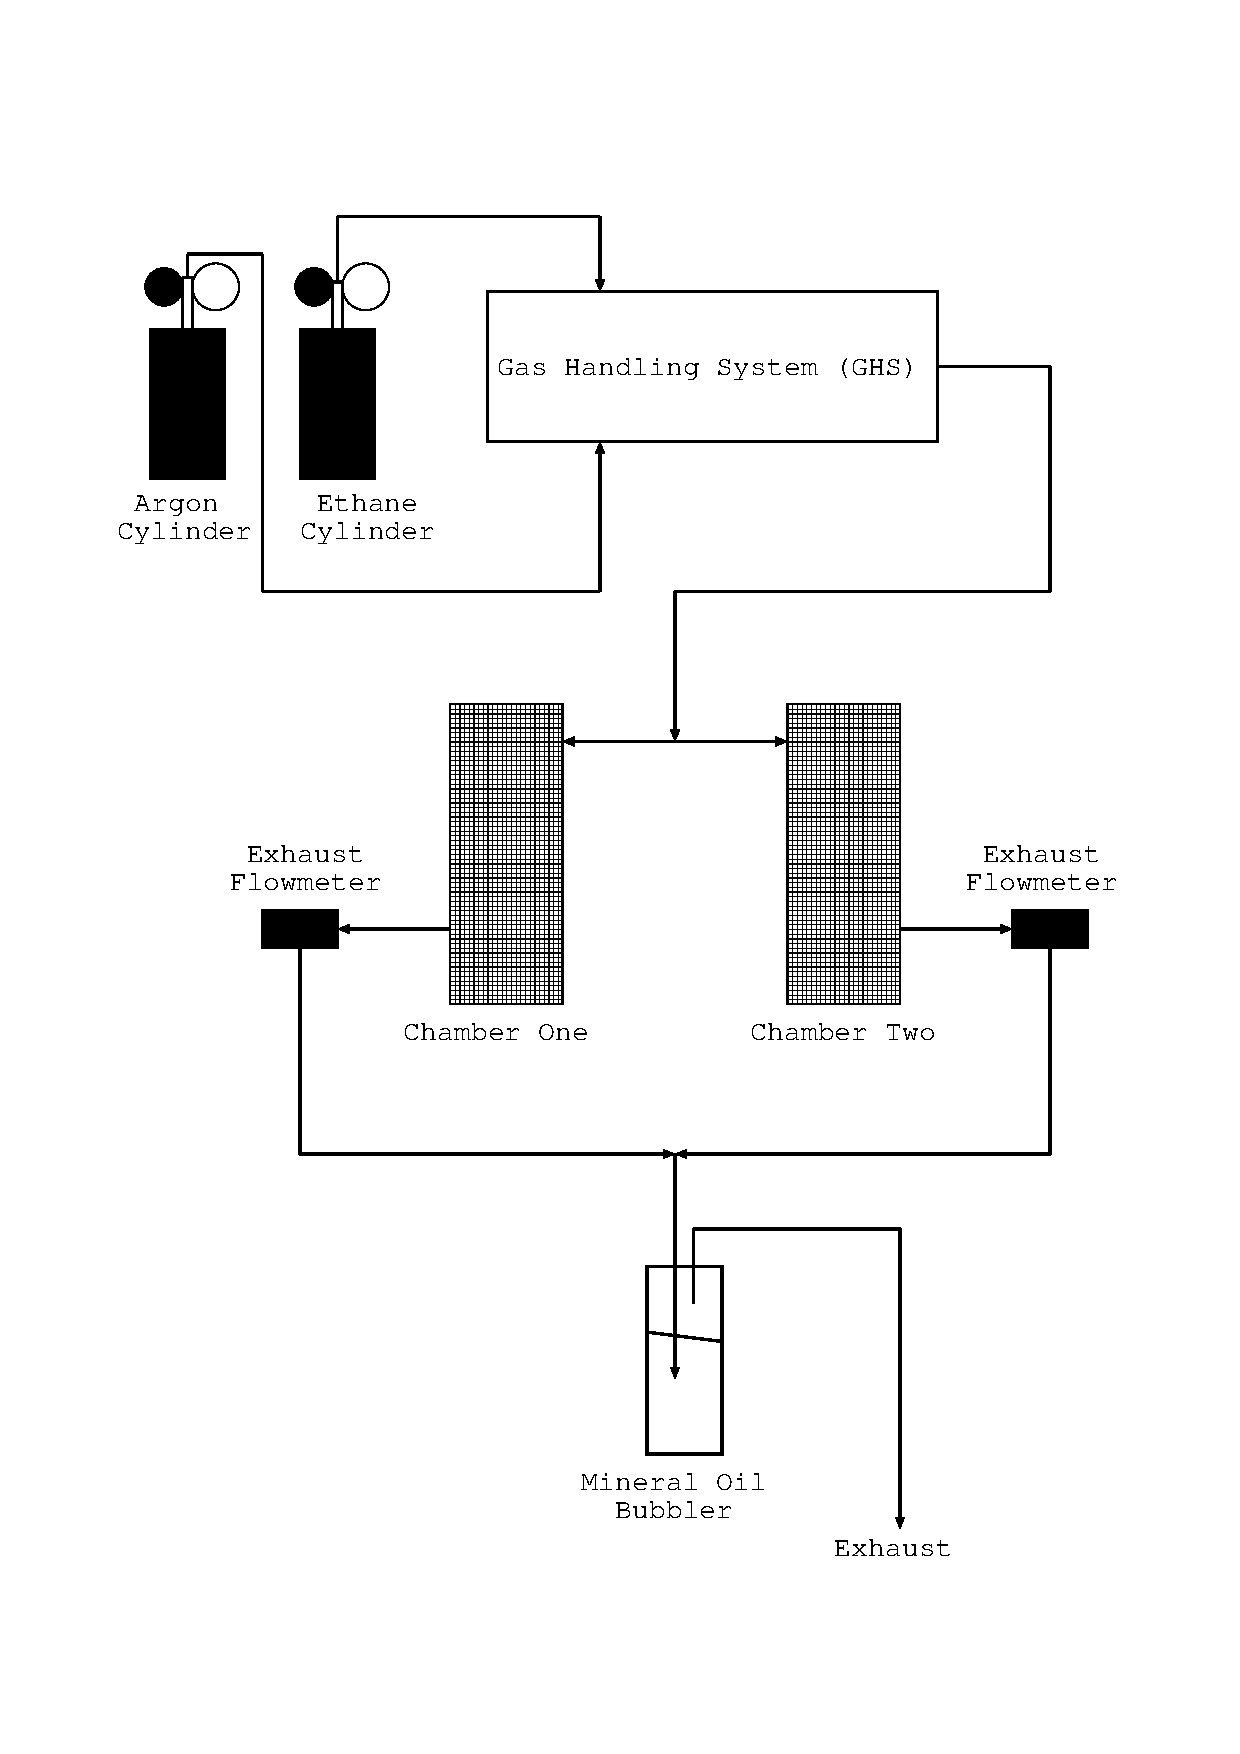
\includegraphics[height=7.5in]{HMSdriftch.pdf}
\caption{The Gas Handling System for the HMS Drift Chambers. \label{fig:5.1}}
\end{figure}

\begin{center}
{\bf Procedure}
\end{center}

\begin{enumerate}
\item {Visually check that the gas flow lines are connected to the two
HMS chambers.}
\item {Check gas pressure and amount in gas cylinders (Ar and C$_2$H$_6$).}
\item {Turn on the gas flow on the MKS controller in the gas hut.}
\item {Set flow through channels three and four to 800 sccm each
(for purging).}
\item {After about 15 minutes, the oil bubbler in the gas hut should
indicate flow.}
\item {The flow rates as read on the flow meters at the chambers should
indicate very low flow (0.3 or so).}
\end{enumerate}

The above settings are for 400 sccm flow through each chamber.  The gas
cylinders should be changed when about 90\% used.  The gas handling system
parameters should be checked every shift (see the checklist at the end of
this document).

\paragraph{Electronics Operating Procedures}

The readout electronics associated with the HMS drift chambers are all
commercial products from LeCroy Research Systems, Nanometrics, Kinetic Systems,
and BiRa Corporation.  There are 544 electronics channels per chamber for
a total of 1088 readout channels.  These anodes are read out using LRS 2735DC
and Nanometrics N-277 preamplifier/discriminator cards mounted directly
on the chambers.  Each chamber has both types of cards, however each plane
(of six total planes per chamber) has only one type of card.  The
digitized signals are sent to FASTBUS TDC inside of the detector hut
via twisted pair cable.  The low voltage (preamplifier) power supplies
(the Acopian supplies)
are in the 13 inch blue rack at the rear of the detector hut.  The
threshold voltage power supplies are on the frame under the Cerenkov
counter.  The remote
threshold power supplies are located in the electronics room of the counting
house.

\begin{center}
{\bf Procedure (in the detector hut)}
\end{center}

\begin{enumerate}
\item {Turn on low voltage power supplies (the Acopian Supplies).}
\item {Turn on threshold voltage power supply to appropriate setting.}
\item {Turn on the FASTBUS power supply if it is not already on.}
\end{enumerate}

It is important that the Acopian power supplies be turned on {\bf BEFORE} the
FASTBUS supplies or the FASTBUS crate will hang up.  The threshold voltage
can be controlled locally in the detector hut or remotely in the
counting house. There is approximately a one volt drop in the threshold
voltage line in going from upstairs in the counting house to
downstairs in the detector hut.  Hence the supplies in the counting
house should be set to 5.5 volts. The local/remote switch is on the
controller in the
detector hut.  It should be switched to remote before exiting the hut.  The
LeCroy preamp/disc cards have LEDs (a green and a red light) which indicate
that the power is delivered properly to the chamber electronics.

\paragraph{High Voltage Operating Procedures}

Only formally authorized person may alter drift chamber high voltage.
There are four different voltages per chamber which must be turned on at the
proper time and monitored throughout the experiment.  {\bf MAKE SURE THAT
GAS IS FLOWING THROUGH THE CHAMBERS AND THAT THERE ARE 
EDGE 
CARDS MOUNTED
ON ALL READOUT CHANNELS BEFORE TURNING ON HIGH VOLTAGE.}  
The high voltage
power supplies are the CAEN supplies located in relay rack CH03B17 in
the counting house electronics room.  The
voltages are set remotely using the GUI in the counting
house. See section \ref{par:hv_ops} for operating instructions.
The four different voltages are (nominally): triangle
wires (corner field wires) (-2500 V),
square wires (-2250 V), circle wires (-1800 V), and guard wires (-1500 V).
Note that each HMS drift chamber {\em plane} has its own triangle, circle,
and square voltage source, while there is only one guard wire voltage
source per {\em chamber}.
\begin{center}
{\bf Procedure (in the detector hut)}
\end{center}

\begin{enumerate}
\item {Make sure a 2735DC card or a grounding plate is on each instrumented
connector on the chamber.}
\item {Make sure that there is gas flow, particularly Ar gas.}
\item {Make sure high voltage cables are properly connected to
chamber.}
\item {Turn on high voltage, using the EPICS GUI in the counting house, 
to proper settings.}
\end{enumerate}

The CAEN power supplies, when operated remotely, are controlled by the
EPICS control system.  To operate, log on to vxworks, get the high
voltage monitors (use the rightmost mouse button to bring up the menu)
and choose the chamber voltage group.  Each high voltage channel is
independently controlled.

In general all of the voltages and gas flow should be left on, even when
no data is being collected.  The gas supply should be checked periodically,
approximately once every shift.  The gas bottles' supply is depleted
after about 2 weeks at the nominal (400 cc/min) flow rate.
In the case of a HV trip, try cycling the CAEN power supplies.  If this fails, call
one of the responsible persons listed in the Responsible Personnel Section 
of the \htmladdnormallinkfoot{ESAD}{http://www.jlab.org/Hall-C/document}.




\subsection{Scintillator Hodoscopes (HMS and SOS)}

The purpose of the scintillator hodoscopes is to provide a clean
trigger as well as particle identification by time of flight (TOF). These
detectors consist of two pairs of spatially separated scintillator
layers: a pair comprised of S1X and S1Y, and approximately 2 meters away a pair
comprised of S2X and S2Y. General characteristics of the BC404 scintillator
material are as follows:

\begin{itemize}
\item{Polyvinyltoluene (PVT) is the base material. }
\item{Light output is 68\% that of Anthracene. }
\item{Wavelength of maximum emission is 408 nm.}
\item{Decay constant of the main fluorescence component is 1.8 ns.}
\item{Bulk attenuation length is 160 cm.}
\end{itemize}

	The specific dimensions for the scintillator elements in the HMS
and SOS are found in Table~\ref{tab:tof_scintillators}.
\begin{table}
\caption{Dimensions (at 70~F.) of the scintillators for the HMS TOF system. 
\label{tab:tof_scintillators}}
\begin{center}
  \begin{tabular}{ccccc}
	&Thickness	&Width		&Length		&Number	\\
	&		&		&		&	\\
\hline
X(HMS)	&	1cm	&	8.0cm	&	75.5cm	&32 units\\
Y(HMS)	&	1cm	&	8.0cm	&	120.5cm	&20 units\\
	&		&		&		&	\\
X1(SOS) &       1cm     &       7.5cm   &       36.5cm  &9 units\\
Y1(SOS) &       1cm     &       4.5cm   &       63.5cm  &9 units\\
X2(SOS) &       1cm     &       7.5cm   &       36.5cm  &16 units\\
Y2(SOS) &       1cm     &       4.5cm   &       112.5cm &9 units\\
  \end{tabular}
\end{center}
\end{table}
Each scintillator is read out by two Philips XP2282B photomultiplier
tubes (PMT's). These PMT's are 8-stage tubes with nominal operation at
2500 volts. The bases have two anode outputs, one of which is terminated with a
short clip line and 40 Ohms.  Because of pmt to pmt variations in gain and the
5\% precision zener diodes in the bases, the spread in gains can be a factor of
2-3. Individual high voltages must therefore be adjusted to balance the gains.
The gains have been carefully matched with a source, and HV save files exist,
so the gains will not normally need to be readjusted. If gain adjustment is
necessary, inform one of the hodoscope contact persons as soon as possible.
Mysterious gain shifts are probably due to transient problems like bad solder
contacts or broken glue joints. They require repair. A rough rule of thumb is
that an increase of 50 volts will increase the gain by 30\%.

With our base, the HV channel will trip on overcurrent (3 mA) at 2900 V
(this base is essentially divider C in the Philips catalog). If a channel needs
more than 2800 volts, and the base and glue joints are okay, then our policy
is to replace the pmt. We have several spare modules in the counting room.
In desperation, ``spares" can be taken from the edges of the acceptance. In the
HMS, S1X16 or S2X16 contain little or no useful data, and similarly for S1Y01
or S1Y10.

	The light guide material is UVT lucite.  Wrapping material for the SOS scintillator elements was one layer of 
aluminized mylar (aluminum side facing inward), followed by two layers of
tedlar for light tightness. The HMS elements were wrapped in aluminum foil,
followed by one layer of tedlar.

	The SOS hodoscopes are mounted in aluminum frames, with brackets over
the lightguides and holders supporting the elements also at the tube/base
assembly. The SOS y-counters are EXTREMELY delicate at the glue joints
connecting the angled light guide with the flat section, due to the geometry.
The HMS elements are supported at the lightguides. In case of repair use BC-600
glue. Each element has a 1 mm plastic fiber glued into the light guide. These
fibers are also very delicate and care must be taken when moving a scintillator
element to avoid snagging and breaking the fibers.

{\bf What to check}: Before starting to operate the detectors, one has to
check the trip setting (current limit) of the HV power supply for each channel
and the set HV value of each channel. During operation, the current of each
channel and its HV should be periodically checked. The HV should be on for at
least half an hour before taking data. During runs one should check the
histogram of the plane hit distribution. This should be rather flat reflecting
the normal trigger requirement of 3 out of 4 planes. Also the element hit
distributions for the individual planes should be checked regularly. These
distributions are defined for both ends of the elements using both ADC and TDC
information.

{\bf Nomenclature}:
The coordinate system (right handed, following TRANSPORT
convention) is defined as z downstream, x pointing down, and when looking
downstream, y to the left. In this convention the X-tubes at positive Y are
called X+ and the Y tubes at the bottom (pos x ) are called Y+. Numbering of
the elements is done as one would read a book in English: left to right in the
case of the Y and top to bottom in X.

	There are one ADC and one high resolution (25 ps/channel) TDC per PMT.
For the SOS, S1X and S1Y and S2Y each have 18 channels, while S2X has 32 making
it 86 channels in total. Each ``X''plane in the HMS has 32 and each
``Y'' has 20, making it 104 channels in total.

	The signals are carried on an RG-8 size cable which is a Belden 213
equivalent. The nominal specifications are 50 Ohm impedance and the signal
velocity is 0.82c . The signals are passively split in the counting house with
one going to the ADC and one going to leading edge discriminators. The
performance is typically 100 and 150 psec mean time resolution (sigma) per
element for the SOS and HMS, respectively.

\subsection{Gas Cerenkov Detector}

A charged particle travelling faster
than the speed of light in the medium will create an electromagnetic
disturbance in the medium. The radiation emitted by this process is
called Cerenkov radiation after its discoverer.

Cerenkov radiation is conically distributed about the trajectory of the
particle, with an angle given by
$$
	\cos{\theta} = \frac{1}{\beta n}
$$
where the index of refraction $n = c/u$ and $\beta = v/c$, with $c$
the speed of light in vacuum, $u$ the speed of light in the medium,
and $v$ the speed of the particle.

The index of refraction allows one to control the threshold particle velocity 
$v_{T}=u=c/n$ below which there is no Cerenkov light produced, and above which there 
is Cerenkov light produced.  For a gas, the quantity $n-1$ is proportional to the pressure, 
so adjusting the pressure of the gas allows one to select the
threshold velocity. Adjusting the threshold velocity actually allows one to select particles of
different mass.  Given the same momentum, two particles of different mass
will have different velocity.  Therefore, a Cerenkov detector can be tuned,
for instance, to distinguish electrons from pions.

	The HMS Cerenkov detector consists of a large cylindrical
tank, $\phi_{in} = 59"$, $L = 60"$, containing two mirrors which focus
light onto two 5 inch Burle 8854 multiplier photo  tubes (PMT's). The tank
has been installed with 0.04 inch thick 2024-T3 Aluminum windows
covering the circular ends of the cylindrical tank. These
windows were hydrostatically formed (and hence tested) at a pressure
of 28 PSI. The tank itself was helium leak checked and is leak free
on a scale of 10$^{-8}$ Atm-cm$^3$/s. In addition, the tank was hydrostatically
tested at a pressure of 35 PSI. Detailed information on this testing
program can be found in \cite {bi:tank}, \cite {bi:wind}.

The tank is mounted on the detector rails using a three point
alignment scheme. The rails are easily capable of supporting the
weight of the tank without deformation.  
The gas handling system for the tank
is designed to enable the tank to be filled with
pure gas, CO2 or N$_2$, at the desired operating
pressure which is, $\approx$ 1 Atm (11.5 PSI) for the near future.

The system consists of the fill gas bottle and primary
pressure regulator which are in a bottle rack that's welded to
the bottom of the HMS detector hut on the small angle side at a height
of about six inches from the hall floor. The primary regulator is
a Matheson model 2596 with a maximum outlet pressure of 400 PSI.
During fills this regulator should be set to 150 PSI.
The outlet of this pressure regulator is connected to the
main gas control panel which is mounted on the first floor balcony
of the detector hut behind the dipole control racks. All connecting
tubes in the system are 0.25 inch diameter stainless steel tubing with
the exception of the nitrogen purge line which is thick wall tygon.
At the entrance to the gas panel there is a 0-300 PSI gauge so that
the pressure in the inlet line can be viewed by the operator.
The line is then relieved by a Circle Seal relief valve set at 200 PSI.
After this, the gas passes through a second regulator (Matheson 3420)
which has an
outlet pressure range of 0-60 PSI. This regulator can be set at
up to 40 PSI for high flow during the early stages of fills
(the line is relieved further downstream by a second
Circle Seal relief valve set at 45 PSI) and then reduced as
the desired operating pressure is approached. Following the second regulator
and its relief valve the gas passes through oil and oxygen filters.
A 120 Volt AC solenoid valve (ASCO) switched with a solid state
relay is used to isolate the gas flow from the tank. The state of
the relay and hence the valve is indicated by a LED on the panel.
The gas line is routed through an opening in the floor of the detector hut
to the tank inlet. A gauge on the panel allows the operator to view
the pressure in the inlet line (the same as the tank pressure
when the subsequent manual valve is open, see following).
At the inlet there is a pair of manual valves (NUPRO)
which allow the fill line to be purged.
During operation the valve which vents the
line to atmosphere is closed and the valve to the tank inlet is open.
The tank is relieved by a 1 inch diameter, 1 PSI pop off (NUPRO) which was
sized to take the
maximum flow of the second regulator even if that regulator has failed
wide open. There is a pressure gauge on the tank so that its condition
can be determined by workers in the shield house. In addition,
there is a Omega pressure transducer (PX-305-05A) and a temperature
transducer attached to the tank. These are read out and powered by
units (Omega) which are located below the gas panel.  Outputs of these
are currently viewed with a video camera attached
to a monitor in the counting house.

Before filling, the tank is first cleaned by executing several pump
and purge cycles. The pump that is used to evacuate the tank is located on a
platform welded to the small angle side of the shield house balcony
which can be accessed from the small angle side of the HMS carriage.
Eventually, it will be possible to switch the power for this pump
from the gas control panel with a relay but currently it
is necessary to turn the pump on and off with a switch located on the pump.
The low pressure side of this pump is equipped with a liquid nitrogen
cold trap to prevent any contamination of the tank (or mirrors !)
with pump oil. This trap will remain filled for approximately
12 hours and should always be checked before use. There is currently
a manual valve located at the Cerenkov tank that isolates the tank from
the pump.  This valve will later be replaced by a pneumatically actuated
solenoid valve that will be controlled from the gas panel.
There is a manual valve on the tank which is equipped with a hose
barb through which clean nitrogen purge gas can be admitted to the tank.
The nitrogen gas comes from a spigot on the HMS cryogenic handling system
located along the upper catwalk of the HMS. The nitrogen system
delivers gas at a line pressure of $\approx$ 40 PSI (this pressure can
be read on a gauge at the pivot end of the catwalk). The flow
rate is readable from a flow meter attached to the spigot. A flow of
about 150 - 200 cfm is reasonable. The tank should not be filled to
more than -5 in Hg during purge cycles.

The tank contains two 5 inch PMT's which use {\bf positive} HV.
Note that all the other PMT bases in the HMS are designed for use with
negative HV. They operate
at between 2000 and 2700 Volts. The Anode is at HV and its signal is
viewed through a decoupling capacitor in the base. The HV is supplied
by one pod of the same {\em CAEN} power supply used for the drift chambers.

The mirrors in the tank may require adjustment for optimal focusing
on the PMT faces. The ports which hold the PMT's are sized big enough to allow
a person inside the tank to make these adjustments. The tank is a confined
space and hence this activity represents an ODH hazard. Stickers indicating
this have been placed on the PMT ports. Before an entry into the tank the
atmosphere in the interior must be surveyed by a member of the physics
division EH$\&$S staff.
This adjustment should only
be done by personnel who understand the fiducial markings of the PMT
mounting system. The interior of the tank has foot braces and hand holds welded
to allow this work at the angle of the detector rails.

\paragraph{Operation Procedures}

\begin{figure}
%\GHS
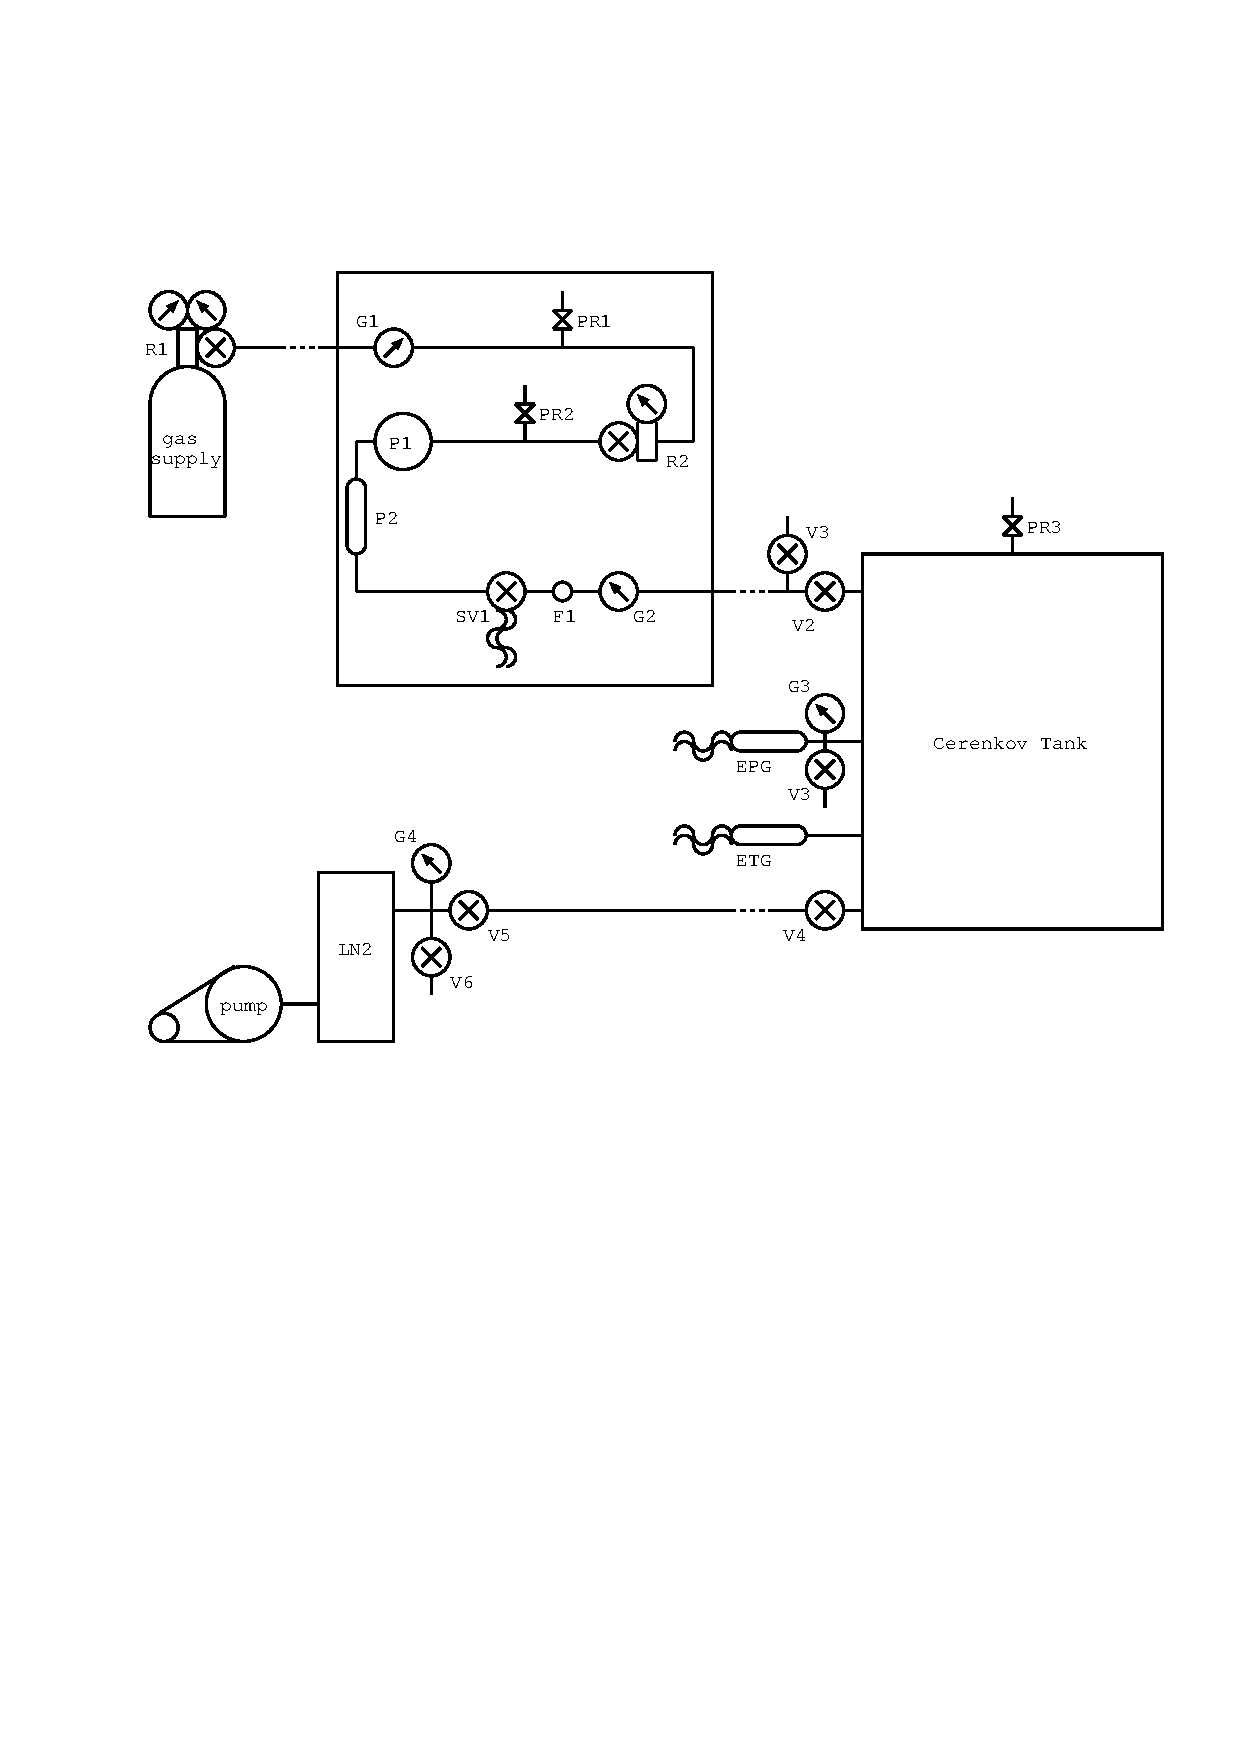
\includegraphics[height=5in,width=6in]{HMSgasC.pdf}
\caption{The Gas Handling System for the HMS \Cerenkov\ Detector. \label{fig:gas}}
\end{figure}

The HMS \Cerenkov\ Detector operates either as an e/$\pi$ or $\pi$/p
discriminator. Each mode has a unique set of procedures to prepare the tank
for operation. The nomenclature used in the description of these operation
procedures refers to Figure~\ref{fig:gas}, showing the gas handling system. Components 
shown
inside the dashed box of Figure~\ref{fig:gas}, are all located on the Gas Control Panel.

\paragraph{e/$\bf{\pi}$ Procedures}
For both e/$\bf{\pi}$ and p/$\bf{\pi}$ separation, the procedure 
has been to run with 0.4 to
0.9 (?) atmospheres of C4F10.  This is just a small modifiction to the
current p/pi procedures write-up described in the next section,
with the HMS running sub-atmospheric instead of supra-atmospheric. 

e/$\bf{\pi}$ running can also be accomplished using a nitrogen fill.
This mode of operation requires the tank to be filled with approximately
13.5~psia of $\rm{N_2}$.  The boiloff from the spectrometer magnets is a
perfect source of clean, dry Nitrogen, and is normally used to fill the
\Cerenkov\ tank.

Because the operating pressure is slightly subatmospheric, a pump and fill
procedure is employed.  First make sure that:
\begin{itemize}
\item The 40~mil windows are installed and oriented such that they curve
towards the interior of the tank.
\item Valves {\bf V1-V6} are closed.
\item The LN2 trap is filled.
\item There is enough oil in the pump.
\end{itemize}
The tank is now ready to be evacuated.
\begin{itemize}
\item Turn on the pump.
\item Slowly open {\bf V5}.  This evacuates the pump line.
\item Very slowly open {\bf V4}.  Since this valve connects the pump line to
the detector volume, the pump will work very hard.  Meter this valve
so that the pump is never under extreme stress.  It will take approximately
20~minutes to pump down the tank.
\end{itemize}
The tank can now be filled.
\begin{itemize}
\item Locate the boiloff manifold on the walkway on the top level of the
spectrometer, at the gap between Q3 and the dipole.
\item Turn the valve on this manifold open slightly so that the flow meter
barely registers a flow.
\item Connect the remaining end of the Tygon tubing to the vent of valve
{\bf V3} with a hose clamp.
\item Open valve {\bf V3}.
\item Increase the flow on the flow meter.  Do not exceed 100~cfpm.
\item When {\bf G3} or {\bf EPG} reach the operating pressure, close
the manifold valve.
\item Close {\bf V3}.
\end{itemize}
The fill should take approximately 30 minutes.  The detector should NEVER
be left unattended during a fill.  Frequently check the pressure in the tank
and be aware when the pressure nears one atmosphere.  DO NOT let the pressure
exceed one atmosphere under any circumstances; doing so risks damage to all of
the equipment and personnel in the detector hut.  This pump/fill procedure is usually 
repeated at least once to insure the
purity of the gas.

\paragraph{$\bf{\pi}$/p Procedures}
This mode of operation typically requires the tank to be filled with Freon-12
at pressures varying from 2 to 3~atm.  Because these operating pressures are
greater than 1~atm, the detector must be filled by dilution.  Contamination
from air, however, is not a major problem as the optical absorption properties
of air are actually more favorable than those of Freon-12 itself; the only
difficulty is the increase in pressure needed for a mixture of air and Freon
to achieve the same pion momentum threshold as for a pure sample of Freon.

First prepare the gas handling system:
\begin{itemize}
\item Make sure that the 60~mil windows are installed and oriented such that
they bulge outwards from interior of the tank.
\item Close the valves {\bf V2-V4}, and the valve on regulator {\bf R1}.
{\bf V1}, {\bf SV1}, and the valve on regulator {\bf R2} should be
open.
\item Open the valve on the gas supply bottle.
\item Adjust {\bf R1} to approximately 60 psig.
\item Open the valve on {\bf R1}.
\item Check to make sure gauge {\bf G1} agrees with the pressure setting
on {\bf R1}.
\item Adjust {\bf R2} so that a small flow is detected out the vent of
{\bf V1}.
\item Close {\bf V1}.
\item Adjust {\bf R2} to regulate at the required operating pressure.
\end{itemize}
The tank is now ready for the dilution process.  These steps should be
repeated as few times as possible to minimize the quantity of Freon-12 emitted
to the atmosphere.
\begin{itemize}
\item Record the tank pressure.
\item Open valve {\bf V2}.
\item Monitor the gas pressure until it reaches the required operating pressure.
NEVER let the pressure in the detector exceed 3~atmospheres.
\item Record the final pressure.
\item Open {\bf V3} to vent the tank.
\end{itemize}
From the recorded pressure readings, the threshold momentum of the mixture
of air and Freon-12 can be calculated (assuming the volume of the tank is
fixed).



\subsection{Lead Glass Shower Calorimeter}

The lead glass shower calorimeter consists of four stacks of
TF1 leaded glass (similar to SF1). Each stack contains thirteen
blocks for a total of 52 blocks. The blocks are 10 cm by 10 cm by 70
cm and all are read out by a PMT at one end at least.  Currently the
two layers have PMT readout at both ends.

High energy particles
emit Cerenkov radiation when passing through the glass and a signal
is collected that is proportional to the sum of the path lengths
travelled by all the
particles which are above the threshold for Cerenkov emission. High energy
electrons will produce a large signal as they have a large bremsstralung
cross section and the photons which are produced in the bremsstralung
process have a large cross section to produce electron positron pairs
(all of which will be above the Cerenkov threshold). This process
of bremsstralung followed by pair production is called an electromagnetic
shower.

The histograms associated with the calorimeter should be inspected
regularly to assure that it is functioning properly.


\section{SOS Detector Package and Shield House }

The detector package is the key to a successful experiment. Its proper
operation should be continuously monitored during the experiments.
There are a large number of diagnostic type spectra available to aid in
this monitoring.
All the detectors are in the shield house (also referred to as detector hut).
The (concrete) shield house protects the detectors from the typical large
background environment associated with a high energy electron beam
traversing through materials (target, exit windows, possible scraping, dump).

\subsection{Shield House and Shield House Door}

The shield house interior access is covered by a two piece door. The two
halves counterweight against each other, opening vertically. The bottom
door (30 tons) is 5 tons heavier that the top door. Thus, the door will want
to open naturally if unconstrained. The door control system is used to keep
the doors closed.

The valves in the control system are set by a PLC that resides in a box
mounted beneath the stairs at the rear of the spectrometer. The front panel
of this box has two buttons for control of the door (Open \& Close),
switches for main power \& the two pumps, and several status lights. The
status lights indicate when it is necessary to clean one of the several oil
filters. The door is designed to operate electronically via a control box
mounted along the walkway near the door or from the panel beneath the
stairs. Indicator lights in the various buttons on the control box
illuminate to show the current status.

\begin{description}
\item{\bf Open} Opens the door, electronically activating the hydraulics.
Pressing this switch will illuminate both buttons on the operator panel and
on the
control box. The door will require about 60 seconds to open.
\item{\bf Close} Closes the door, electronically activating the hydraulics.
Pressing this switch will illuminate both buttons on the operator panel and on
the control box. The door will require 60 seconds to close.
\item{\bf Emergency Open} Used only if the hydraulic system fails but electrical
power is available. (i.e. hydraulic pump failure) This button operates
valves so that hydraulic fluid slowly exits the door cylinders and allows the
doors to open. Opening the door this way may require several minutes.
This switch is not spring loaded and will have to be manually reset before
other operations can continue.
\item{\bf Emergency Stop} Stops the movement of the door regardless of
direction.
This switch is not spring loaded and will have to be manually reset before
other operations can continue. Resetting the switch does not resume door
motion. Another button must be pressed to start movement again.
\item{\bf Standby} Once the door is stopped, standby may be used to keep
the door
within 0.5" of its' present position. This switch is disabled during door
movement. If the doors creep through fluid leaking by the seals in the
cylinders while the system is in standby mode the pumps will activate and the
slippage will be corrected. The cleaner the system and newer the cylinder
seals the less this slippage will occur.
\end{description}

The circuit for the door controls is located in boxes C-UPH3 (pumps, circuits
20,22,24) and C-UPL3 (120V, circuit 35).

The control panel controls:

\begin{description}
\item{\bf Open} Same as above.
\item{\bf Close} Same as above.
\item{\bf Large Grey power switch} Switches on power to electronics and pumps.
\item{\bf Pump 1, Pump 2} Each pump may be enabled individually. These two
switched do not start the hydraulic pumps.
\item{\bf On} Starts the enabled hydraulic pumps.
\item{\bf Off} Stops the enabled hydraulic pumps.
\end{description}

\subsection{Opening/Closing SOS Shield House Doors}

To open SOS shield house doors, first confirm appropriate breakers in
breaker panels on right side of carriage are "on". Open doors on power
panel at right rear of carriage, then close right hand door, making sure
that switch handle on outside of door engages switch shaft. Leave left door
open.
Operate switch handle to turn on 480 volt power. Watch message panel on
orange plc box near left end of top row of modules. Message panel should be
blank. If any message appears, {\bf STOP} and call/page Hickson or
Vulcan.  If panel is
blank, proceed. On exterior of right hand door, select either pump \#1 or
pump \#2, then press green "on" button below pump selector switches. Note
sound of pump. Go up S.O.S. stairs to walkway in front of doors. Insert
enable key in control box, and turn to "on" position. Press and hold "open"
button. Button must be depressed for - 5 minutes, 40 seconds to open doors
completely. While opening doors, watch door hydraulic cylinders; cylinder
movement should be synchronized. lf differential movement is observed,
release "open" button, hit "emergency stop'' button and call/page as 
above.  Doors will stop automatically at full open position.
If doors will be open for more than a few minutes, return to floor level
power panel and turn pump off with red "off' button below pump selector
switches, then turn off 480 volt power with switch on exterior of right
hand door. If pump is left on, close doors by pressing and holding "close"
button for - 5 minutes, 40 seconds. Doors will stop automatically when
fully closed.  When doors are closed, turn enable key to "off' and remove
key from control box. Return to 480 volt panel, turn off pump, and turn off
480 volt power. If 480 volt power was turned off while doors remained open
for an extended period, 480 volt power must be turned on to close the doors
as described above. Always observe message panel on plc after turning on
480 volt power. Never proceed If any message is displayed.

NEVER LEAVE 480 VOLT POWER ON DURING BEAM PERMIT.

NEVER USE "STANDBY" MODE.



\paragraph{Safety Items}

With the loss of electrical power all valves close automatically. This will
stop all movement of the door. The fluid in the cylinders may slowly leak
past the seals causing the door to open.

A section of handrail will be (is) attached to the downstream end of the
flip-down section of walkway. This handrail will block access to the doors
until the doors open completely and the flip-down walkway can be rotated
over the lower door.

The toe kick around the roof of the shield house will be (has been)
extended to 8", and sealed to contain fluids in the event of a catastrophic
hydraulic leak. The enclosure should capture 330 gallons of fluid adequate
to contain a complete system rupture.  The most common mode of fluid
loss is a slow drip at a joint. Rupture of a hose, while very unlikely, can
result in loss of fluid in that hose. Pressure indicators in the system
will stop
the system if loss of pressure is detected. See the hydraulic diagram for
the location of the pressure indicators (Figure~\ref{fig:SOSdoorHydSym}: explanation of symbols,
and Figure~\ref{fig:SOSdoorHydDiag}: the hydraulic diagram).

Filter replacement is required when the maintenance light on the control
panel is illuminated. The filter elements are placed between two isolation
valves. The two valves must be closed, and the pressure released before
the filter cover is removed. The filter cover is a screw on/off type. The
elements are not disposable and are designed to be cleaned and replaced.

\subparagraph{Filter Removal}

\begin{enumerate}
\item{Turn off the power to the control system.}
\item{Close the valves on either side of the filter to be replaced.}
\item{Release any built up pressure in the filter and neighboring pipe by
opening the pressure relief needle valve at the filter. Be careful of any fluid
released through the valve. {\sl The released fluid should be captured and
disposed of properly.}}
\item{Unscrew the filter cover.}
\item{Service the filter.}
\item{Replace the filter and cover.}
\item{Close the pressure relief needle valve.}
\item{Open the valves on either side of the filter.}
\end{enumerate}

\subparagraph{Valve Failure}

The solenoid valves have lifetimes of many thousands of cycles.
In a valve fails, the two pressure indicators will start to differ, soon
resulting in a too large difference between the two decoders (one for each
side of the door), causing the motion mechanism to stop.

\subparagraph{Cylinder Failure}

In the unlikely event of a cylinder failure, the door will slip slightly to one
side in the track and any motion will stop.

\paragraph{Manual Door Operation}

In the event that electrical power is lost (and thus hydraulic control) the
door can be opened manually. There are five manual popet valves, that are
to be opened in a certain sequence, that will allow hydraulic fluid to slowly
drain from the cylinders thus opening the doors.

\begin{enumerate}
\item{Open the popet valve at the top of each door cylinder (valves SV-C-9
\& SV-C-10) by
pressing the switch on the valve. The valve is located on the downstream
side at the top of each cylinder.}
\item{Open the popet valve at the bottom of each cylinder (valves SV-C-11
\& SV-C-12) in
the same way. The valve is located on the upstream side at the bottom of
each cylinder.}
\item{Finally open the valve (valve SV-C-13) located on the rear wall of the
spectrometer, above the electronics hut.}
\end{enumerate}

The fluid drains from the cylinders slowly. Opening the door this way may
take more than several minutes. The five solenoid valves will need to be
reset before electronic operation can resume.

\subparagraph{Pump Failure}

The hydraulic pump has two motors that are independently switched.
Either will provide adequate power to operate the SOS door hydraulics. It
is recommended that both pumps be used or alternated so that both are kept
lubricated.

The motion of the door is monitored by the control system. Linear
displacement encoders on each cylinder provide analog signals to the controls.
The two cylinders must move at the same rate or the control system will
stop the door progress. The doors will stop if the difference between the
cylinders becomes more than 0.020". The control system will attempt to
level the door and continue, massive skewing of the door will cause the
door to wedge in the track. If the door wedges in the track crane support
may be necessary to correct the problem.


\begin{figure}
%\htmlimage{scale=2.0,thumbnail=0.5,flip=r270}
\includegraphics[height=7.2in,width=6.25in]{SOSdoorHydSym.pdf}
\caption{Explanation of Symbols used in Door/Jack Hydraulic 
Diagram. \label{fig:SOSdoorHydSym}}
\end{figure}
\clearpage

\begin{figure}
%\htmlimage{scale=1.0,thumbnail=0.5,flip=r270}
\includegraphics[angle=270,width=6.25in,totalheight=7in]{SOSdoorHydDiag.pdf}
\caption{The SOS Door/Jack Hydraulic Diagram. \label{fig:SOSdoorHydDiag}}
\end{figure}
\clearpage


\subsection{High Voltage Supplies }

All the detector elements require the use of High Voltage. The
high voltage supplies for the detectors are located in the 
electronics room of the counting house.
During experiments the control of the high voltage supplies is done via
computer and a display is available on one of the xterms around
the console in the Hall~C counting house. The control is via
EPICS and includes a graphical display so that the status of each
HV channel can be seen at a glance. Operating instructions are
in section~\ref{par:hv_ops}. {\em Typical} high voltages for
SOS detector elements are shown in Table~\ref{tab:sos_hv}.

\begin{table}[!hbt]\centering
   \caption{SOS Detector {\em Typical} High Voltages\label{tab:sos_hv}}
   \begin{tabular}{lrr}
      Detector & Voltage (V) & Current (mA)\\
      \hline
      Lucite         & 3000  & 1.0 \\
      Aerogel        & 2590  & 1.2 \\
      Gas Cerenkov   & 2875  & 2.2 \\
      Scintillators  & 2500  & 2.1 \\
      Shower Counter & 1350  & 2.1 \\
      \hline
   \end{tabular}
\end{table}

As a general rule no work should be done on detectors which are under
High Voltage and
High Voltage cables should never be removed or installed while the supply is on.
General information about the use of the {\em CAEN} power supplies can be
found earlier in this chapter.


\subsection{Drift Chambers}

\paragraph{Overview}

The drift chambers provide accurate measurements of the particles
position and angles in the detector hut. This information can be combined
with a knowledge of the spectrometer optics to infer the trajectory of the
particles at the target.

The multi wire Drift Chamber module consists of six planes of gold-plated
tungsten wires of two thicknesses: 30 $\mu$ wires held at ground
potential, and 60 $\mu$ wires held at high (negative) potential
($\left|V\right|\le3$kV).  Alternating with the wire planes are six
foil planes of 1/2 mil mylar, coated on both sides with 1200 angstroms
of copper.

The high voltage (HV) system provides the correct potentials on the
cathodes (field wires and foil planes) of the DC modules.  The HV
system is supplied by CAEN high voltage, low current power supplies.
The supplies are located in the electronics room of the counting
house. They are connected to the detectors through a high voltage patch
system from the counting house to the shield house
and coaxial cables with standard SHV connectors from the patch system
to the drift chamber modules.
The highest operating voltage in use presently is -2100 V.

Each anode wire has its own electronic readout through
Nanometrics preamplifier/discriminator
cards or LeCroy Corporation LRS 2735DC cards which are interchangeable
with the Nanometrics cards.  Each of these Drift Chamber cards has 16 inputs
which accept negative signals from the anodes (sense wires), amplify
and then digitize the signals according to whether a user-specified
threshold level is crossed.  This threshold level is set using a low
voltage (0 to 10 volts) dc power supply.  A
multi wire cable connects this threshold power supply to the Drift Chamber cards.
Each of the Nanometrics or LRS cards requires approximately five volts
(bipolar) and approximately 1/2 A.  This power is supplied by Acopian
supplies.  Each discriminator
output is connected by 34-pin (17 pair) twisted-pair cable to an LRS
1887 96 channel pipeline FASTBUS TDC.

The chambers use a 50:50 mixture (by weight) of
argon and ethane gas.  The gas is mixed in a specially-built Gas
Handling System which passes the mixed gas through an alcohol (ethanol) bubbler before
passing it to the chamber.
The gas flow is approximately 100 SCCM.

\paragraph{Personnel and Troubleshooting}

There are not many problems associated with the chamber that are
easily diagnosed from within the counting house.  The main problems
that can be addressed are empty gas bottles (replace them) and tripped
voltages (reset them). All permanent members
of the Hall~C physics and engineering staff may change gas bottles.
If the gas lines become clogged, the high
voltage should be turned off; however, there is currently no way to
monitor the gas flow without going into the detector hut.
Consequently, the gas flow should be checked during routine entries.
If the gas is not flowing, one of the lines is probably clogged.
Contact one of the SOS chamber experts (listed in the Responsible Personnel
section of the 
\htmladdnormallinkfoot{ESAD}{http://www.jlab.org/Hall-C/document})
 for further instructions.

\paragraph{Gas Flow Operation Procedures}

The gas used in the SOS drift chambers is a 50-50 mixture (by weight)
of argon and ethane.  Each chamber has a volume of approximately 13
liters, and is operated at slightly above atmospheric pressure.  When
the gas is flowing through the chambers, the windows of the chambers
will bow out slightly.

The gas bottles sit immediately outside the gas shed, which is outside
the counting house.  The pressure in the argon bottle should be
monitored daily; when it reads below 500 psi, the bottle should be
changed.  Since the ethane bottle contains compressed (liquid) ethane,
the pressure reading is not directly useful.  However, the bottle sits
on a scale.  An empty bottle weighs approximately 120--140 lbs.  When
the weight of the bottle approaches this value, the ethane bottle is
nearly empty and should be changed.  Note that since ethane is a
flammable gas, the regulator on the bottle has reversed threads.  Full
bottles of both argon and ethane should be in the same area as the
bottles in use.  

Normally, Hall C technical staff routinely checks gas bottles and
replace empties.  Experimenters are responsible for verifying and
recording gas status.  

The gas handling system (GHS) is located inside the gas shed.  It
mixes the argon and ethane in the desired proportion, and bubbles the
mixture through alcohol at 0$^\circ$C before the gas goes down into
the hall.  There are four ``channels'' (gas lines) in the system;
channels 1 and 2 are for SOS, and 3 and 4 are for HMS.  The channel is
selected with the left/right arrow keys.  The selected channel may be
turned on or off with the up/down arrow keys, which perform the same
function.  {\em Note that the on/off buttons do not control whether
the gas is on or off}.  Changing the gas flow is accomplished by
moving the cursor to the setpoint value of interest, and typing in the
desired value on the numeric keypad.  Typical values used for SOS are
200 SCCM.

To turn on the gas to the SOS drift chambers, use the following
procedure:

\begin{itemize}
\item{Ensure that the gas lines are connected to the chambers.}
\item{Ensure that the gas bottles are full.}
\item{Turn the gas flow on for channels one and two.}
\item{Set the gas flow on both channels to 200 SCCM.}
\item{After a few minutes, verify the flow rates on the flow meters at
      the chambers of 0.1--0.2 liters/minute.  If this is not the
      case, one of the gas lines is probably clogged.  See the {\em
      Troubleshooting} section for more details.}
\end{itemize}


\paragraph{High Voltage Operation Procedures}

The high voltage for the SOS drift chambers is supplied by a CAEN
high voltage power supply in the electronics room of the counting
house.  The voltage is controlled using the
high voltage GUI running on an  X-terminal in the counting house.
Instructions for using this system are in section \ref{par:hv_ops}.
The operating
voltage for the chambers is 1975V (foil) and 1975V (potential
wires).

At the start of an experiment, first ensure that the gas system is
turned on and gas is flowing through the chambers using the procedures
in the last chapter.  If the system has been off for an extended
period, gas should be flowing for at least 4 hours before high
voltage is turned on.

Control of the CAEN high voltage supplies is performed through
a GUI. See section \ref{par:hv_ops} for operating instructions.

\paragraph{Low Voltage Operation Procedures}

The low voltage for the SOS drift chambers is controlled by two
Acopian power supplies.  One provides +5V, and the other provides -5V.
The two supplies are located on SOS itself, in the level with the
electronics.  The only control on these supplies is an on/off
switch.  For normal operation, both switches should be in the ON
state.  Under normal conditions, with all preamp/discriminator cards
connected, the supply currents are approximately 26A(+5) and 48A(-5).

\paragraph{Threshold System}

The threshold for the SOS drift chambers is controlled by a BK
Precision 1660 power supply, located in rack CH03B10 in the
electronics area.  The SOS thresholds are controlled by the left
module of the lower supply.  The optimal threshold at the operating
point of the chambers is 1.5V.  This is set with a dial on the front
of the device.

\paragraph{Start-of-Run and End-of-Run Procedures}

The procedure for turning the chambers on at the {\bf start of an
experiment} is the following:

\begin{enumerate}
\item{Make sure gas is flowing through both chambers.}
\item{Turn on the low voltage Acopian power supplies in the SOS
      detector hut.}
\item{Turn on the FASTBUS power supply if it is not already on.}
\item{Turn on the threshold power supply to the appropriate setting
      (nominally 1.5V).}
\item{Turn on the high voltage.}
\end{enumerate}

\vskip 0.5 in
{\bf End-of-Run procedure}

At the end of an experiment, the high voltage supplies and the Acopian
power supplies should be turned off.  The ethane gas flow may be shut
off, but the Ar gas flow should be left on.


\subsection{Scintillator Hodoscopes }

See the section on the HMS scintillator hodoscope for more information on the SOS scintillator hodoscopes.  The specific dimensions for the scintillator elements in the SOS
are found in Table~\ref{tab:tof_scintillators}.
Note that the size of the scintillator elements
comprising SY2 is larger than for SY1, to account for the flare of the
SOS acceptance in the dispersive direction.

\subsection{SOS Gas \v{C}erenkov Counter}

See the material on the HMS \v{C}erenkov counter for information on the general 
principle of a gas cerenkov detector.

The SOS Gas Cerenkov Counter distinguishes electrons from pions.  It
is a box, approximately 1 cubic meter in volume, made of 0.5 inch
thick aluminum walls.  There are two end windows each composed of one
layer of 0.010 inch lexan (for gas tightness) and a thin layer of
tedlar (for light tightness).  There are four ports for
photomultiplier tubes (PMTs), six holes for gas I/O, and two 0.5 inch
thick aluminum access windows.  When in operation, the vessel is
flushed with nitrogen and filled with Freon-12 at atmospheric
pressure.

Since the entrance and exit window of the
SOS Cerenkov tank do not allow for a large differential pressure the
tank is filled by the method of dilution.
The differential pressure is measured by means of a differential
pressure gauge.
A video camera is installed such that the reading on this gauge can be
permanently monitored in the counting house.

	The purpose of the remainder of this Section is to give the user
a relatively detailed description of the detector.  Users who need still more
detail are urged to consult the ``JLab Hall~C SOS \v{C}erenkov
Detector Handbook'' as written by W.R. Smythe, University of Colorado
\cite{bi:Smythe}.

\paragraph{Location and Positioning}

	 The gas \v{C}erenkov detector has been installed in the detector
hut of the SOS in Hall~C. The detector is designed to be removed easily
from the sliding detector stand in order to swap the gas \v{C}erenkov
detector with the aerogel \v{C}erenkov detector.  If the detector needs to
be removed, make sure the 4 high voltage cables, 4 signal cables, AC
power for the solenoid valve, the signal/power cables to the meter
camera, and the entrance and exit gas lines are disconnected.

	The mirrors are located symmetrically about the center of the
detector, and as such, the detector is to be centered with respect to
the SOS acceptance.  In X, the vertical direction, the center line of
the tank should be aligned with the beam spots on the wall of the SOS
hut.  This is accomplished by raising and lowering the whole detector
on the four 2'' threaded rods.  In Y, the transverse direction, the
tank should be in line with the center of the beam exit window.  This
should happen automatically as the stand is slid and locked into
place.  See the mirror section for discussion of mirror alignment
within the tank.

	The machine shop drawings of the detector and its stand, the
``boot,'' are located in the drawing cabinet upstairs in the EEL and
also in the SOS Gas \v{C}erenkov Handbook.

	The high voltage supplies for the PMTs are also in the hut and
are under remote computer control.

\paragraph{Gas Handling System}

The Cerenkov tank is manually filled, and topped-off as necessary to
maintain its freon fill.
The tank is maintained at atmospheric pressure through its
connection to a small flexible bladder located on the floor of the
SOS shield house. Care must be taken to prevent any weight or other
force being applied to this bladder (other than its own weight), or
kinking or otherwise blocking flow through the tube connecting the
bladder to the tank.

	A system exists for dynamically maintaining tank pressure but it 
is not normally used:  A relief valve will release at 0.5 PSI
overpressure. Upon an underpressure of 0.2 psi a solenoid valve 
will open, allowing freon to flow
into the tank.  

The solenoid valve is regulated by an Omega Pressure Meter which also
serves to continuously display the current differential pressure in
PSI. This meter is visible on one of the video links displayed in the
counting house.  The tank will normally vary in pressure through +/-
0.05 PSID as the atmospheric pressure changes.  If the tank is
anywhere below -0.1 PSID or above 0.1 PSID, notify one of the
responsible personnel.

	The freon tank is housed in a bottle rack welded to the
beam-side of the SOS carriage.  A gas line then runs up to the detector
hut.  In the event of an overpressure situation, the freon is vented to
the atmosphere via an exit gas line located on the beam side of the SOS.
Freon-12 is a liquefied gas, and a pressure
regulator cannot be used to tell the contents of the bottle as it will
read the fluid vapor pressure up until the bottle is empty. For this
reason the bottle is placed on a scale.

	The DuPont spec. sheet for freon 12 indicates that it takes
approximately 9.4 lbs of freon to fill the tank once.  To fill the
detector with freon, use the manual override switch on the pressure
meter box to open the solenoid valve (a red light indicating the open
valve should turn on).  Also open the manual valve located on the top
of the tank to release the exit gas.  One has to continuously monitor
the pressure meter as a substantial overpressure can occur during a
fill.  A nominal pressure reading during a fill is about +0.07 PSID,
and a continuous tweaking of the freon tank valve is necessary to
maintain this.  The detector is filled from the bottom (freon is
heavier than air), and the
amount of freon admitted is determined by weighing the freon can
during a fill.  30 lbs of freon is deemed to be sufficient for 95\%
freon purity starting from pure air.
Note that the thickness of 1 meter of freon-12 is 0.53~g/cm$^{2}$.

\paragraph{Beam Entrance and Exit Windows}

	The large area windows are fabricated from 0.010'' thick Lexan
graphic film (General Electric Co.).  This film is very strong and
rugged, but it is not quite opaque.  For this reason, a sheet of
0.002'' Tedlar (PVI film, E.I. DuPont de Nemours and Co.) has been
taped to the external surface of the Lexan.  Each foil is clamped
against a gasket cut from a single sheet of 1/16'' neoprene.  The
gasket is first given a light coating of vacuum grease, such as
Apiezon L, on both of its surfaces.  Care should be taken to avoid
tearing the Lexan on the gasket bolt threads when removing/replacing the
windows.

	When tightening the bolts after replacing a window, be sure to
gradually tighten them from a variety of positions (like putting a wheel
on a car) to distribute the force evenly creating a uniform seal.  After
assembly the chamber is usually leak tested.  Approximately 0.5
atmospheric liters of freon 12 is admitted to the chamber, and its
pressure is increased by the addition of compressed air until it is
about 6 torr above ambient pressure.  Then a Yokogawa universal Service
leak detector model H-10G (freon sensitive) is used to check the chamber
for leaks.

	The total thickness of the Lexan/Tedlar windows is 39~mg/cm$^{2}$.

\paragraph{High Voltage}

	Nominal high voltage settings are shown in Table 2.18:

\begin{table}
\caption{HV settings for the SOS Gas Cerenkov Detector\label{tab:sos_c_hv}}
\begin{center}
\begin{tabular}{|c|c|r} \hline
{\em Tube No.} &
  \multicolumn{2}{c|}{\em Voltage} \\ \hline
 1  & 2705 V  \\
 2  & 2641 V \\
 3  & 2571 V \\
 4  & 2687 V \\ \hline
\end{tabular}
\end{center}
\end{table}
These voltages may change and new valves are maintained by the HVPS
database.  They should NEVER EXCEED 2900 volts
without contacting someone from the responsible personnel listed
in the \htmladdnormallinkfoot{ESAD}{http://www.jlab.org/Hall-C/document}!

	The voltages are controlled remotely using the standard CAEN net
connections.  Normal high voltage operating procedures should be
adhered to.  If you need to change the high voltage by more than 20
Volts contact one of the responsible personnel.

\paragraph{Photomultiplier Tubes and Bases}

	The detector employs four Burle 8854 PMTs.  These are large
5'' diameter, 14 stage tubes.  They are housed in magnetic shields,
and look through ``Winston cones,'' parabolic mirrors that ``funnel''
photons to the photocathode.

	{\bf To remove a phototube from the detector, do the following:}

\begin{enumerate}
\item {\em Remember never to touch or apply force to the phototube face.  This
glass/metal seal is very fragile!}

\item  Loosen the hose clamps that connect the phototube and base and remove
the base.

\item  Remove the six brass nuts that hold the phototube flange to the
detector tank.

\item  Remove the whole phototube assembly (tube, flange, Winston cone and
support) taking care not to bump the Winston cone on the hole in the
tank.  The assembly is somewhat ``off balanced'' and a little heavy...  It
has been found that a round ``office'' waste basket is very useful in
supporting this assembly, tube up, on a work bench.

\item  Loosen, but do not remove, the three, small, regular head screws
that hold the Winston cone back against the phototube face.

\item Undo the three allen bolts that connect the aluminum ring (connected
to the back of the Winston cone) to the flange (via the brass rods).
The Winston cone should now be free.

\item Now wiggle the magnetic shield, with the tube inside, free of the
aluminum cylinder and flange.  Take care not to let the phototube fall
out of the shield.  It's a little tight because there is an
O-ring inside that forms the gas seal.

\item  Finally, remove the plastic ring from the face of the tube, and then
remove the tube from the magnetic shield.
\end{enumerate}

	{\bf To replace a phototube, do the following:}
\begin{enumerate}

\item  {\em Remember never to touch or apply force to the phototube face.  This
glass/metal seal is very fragile!}

\item  Place the flange on top of an ``office'' wastebasket with the aluminum
cylinder pointing down.

\item  Insert the o-ring into the back of the wide part of the magnetic
shield, slide the phototube in, and place the plastic ring around the
face of the tube.

\item  Wiggle the magnetic shield into the aluminum cylinder/flange.

\item  Place the Winston cone assembly onto the front of the magnetic
shield.  The three small, regular screws should be loose.  Note that
the shield should catch on the small lip on the inside of the aluminum
ring connected to the cone.  Tighten the three allen bolts that attach
the cone assembly to the flange via the brass rods.

\item Center the Winston cone on the phototube by gently pushing the cone
up against the plastic ring around the phototube.  There is no need to
apply force!  Tighten the small screw holding the cone in place.

\item Once you're sure that everything is secure, pick up the whole
assembly and place it (Winston cone first!) into the detector tank.
Making sure the flange O-ring is inplace, tighten the six brass bolts
slowly, and in a ``star'' pattern.

\item Place the hose clamp collar around the phototube base housing, and
slide it up along the housing such that the white phototube socket is
the furthest thing out.  This will enable you to see the pin alignment
hole as you connect it to the phototube pins.  Once the tube is
connected (take care not to touch the pins, there is a strong argument
that this increases dark current...) slide the hose clamp collar down,
such that it is centered between phototube and base.  Tighten the hose
clamps as needed.  (Note that the center of the phototube and base are
often not quite collinear.  This is normal, and a little bit of
``tweaking'' is necessary.  Try to maintain that fine line between being
gentle and forcing it.)
\end{enumerate}

\paragraph{Mirrors}

	There are four overlapping mirrors that reflect photons to their
respective PMT.  The mirrors consist of a thin layer of aluminized mylar
evaporated onto acrylic backs.  These are then glued to a foam backing
that is connected to aluminum support structures.  (Note that aluminum
supports are ``L'' shaped such that they are on the extreme edges of the
detector and not in the center of the acceptance!)

	A right-handed rectangular coordinate system is employed which
is the same as the defined on page 9 of the {\em Conceptual Design
Report} \cite{bi:Woodin} .  The origin is the intersection of the beam
axis (also the \v{C}erenkov counter axis of symmetry) with the
\v{C}erenkov detector entrance foil.  The positive Z axis coincides
with the beam axis and passes through the center of the exit window.
The X-axis points upwards in the vertical (or bend) plane and the
Y-axis then lies in the horizontal (or scattering) plane.  The four
mirrors are assumed to have radii of curvature of 100 cm (39.4'').
The alignment of the mirrors can be specified by specifying the
location of the center of curvature of each of the (spherical)
mirrors.  The centers are:


$Z=0$

$X=\pm9.64''$

$Y=\pm14.0''$


	This is the approximate alignment arrived at in the Dale
Woodin Conceptual Design Report, and appears to be quite adequate.  In
order to provide overlap and avoid interference, the mirrors have been
offset from each other in the Z direction by small amounts, with
negligible impact on their light collection ability.  The actual
mirrors can be described as rectangular sections (13.8'' x 17.8'') of
a spherical surface.  To locate the centers of curvature correctly,
these mirrors must be tilted away from the Z axis about $11^{\circ}$
in the horizontal direction and about $1^{\circ}$ in the vertical
direction.  Because of the tilt and the curvature of the edges of the
mirrors, the mirrors must be overlapped to avoid gaps.  A mirror
mounting system has been designed which allows the mirrors to be tilted
in the XZ and YZ planes, and to be translated in the Z direction and
in the $11^{\circ}$ plane (approximate Y direction).  The first three
motions are provided by the three screws which attach each mirror to
the mounting frame.  Translation of $\pm0.5''$ is provided in the
``$11^{\circ}$ plane'' by slots in the mirror mounting plate.

	The mirrors are numbered 1 through 4.  They are removed in
order 1, 2, 3, 4 and installed in the reverse order.  The equipment
for checking the alignment of each mirror consists of a source lamp
which can be mounted in place of each phototube in turn.  You will
also need a screen on which the light from the lamp is focussed by the
corresponding mirror.  The source lamp is located on the phototube
axis 4.50'' outside of the phototube mounting port, at coordinates:
$X = \pm9.64''$, $Y = \pm22.69''$, $Z = 7.02''$.  A ray tracing
calculation for reflection from a spherical mirror ($R = 39.37''$)
with its center at $X = \pm9.64''$, $Y = \pm14.00''$, $Z = 0''$
locates the images at $X = \pm9.64''$, $Y = \pm2.9''$, $Z = -1.8''$.
The actual best image with the mirrors installed seemed to be at about
$Z = 4''$.  The mirror mounting screws are adjusted to produce
patterns in the Z=0 plane which were symmetric about the points $X =
\pm9.64''$, $Y = \pm2.9''$.  This was accomplished by only small
changes to the initial settings of the adjustment screws.  Experience
shows that the mirrors can be removed and reinstalled without any need
to reset the alignment, provided that the adjustment screws are not
changed.  Only the plate mounting screws need to be removed to remove
a mirror.

	The total thickness of the mirror assembly (not including the
aluminum; it's on the edges only) is 450 $mg/cm^{2}$.

\paragraph{Online Issues}

	The raw ADC spectra are included in the standard ntuple
generated by the ``engine.''  In addition the detector efficiencies
(and nominal values) are reported in the standard SOS scaler report
files.  More detailed SOS gas \v{C}ernekov diagnostics will be
included in a separate routine.  See the directory
/cdaq1/usr/users/cdaq/documents on the HP UNIX machines for details.


\subsection{Lead Glass Shower Calorimeter }

The lead glass shower calorimeter consists of four stacks of
TF1 leaded glass (similar to SF1). Each stack contains eleven
blocks. The blocks are 10 cm by 10 cm by 70 cm and are read
out at one end by a PMT.

To take the asymmetric flare of the SOS acceptance into account five of the
eleven blocks are placed below the nominal central ray point of incidence,
and six of the eleven blocks are placed above this point.

See the section on the HMS lead glass shower calorimeters for
 more information on the SOS lead glass
shower calorimeters.


\subsection{SOS Aerogel Detector }

The Aerogel detector is used for kaon/proton discrimination.
Aerogel is a very porous glass with an index of refraction of approximately
1.04.
The detector consist of a airtight diffusion box which contains the
Aerogel and fourteen Burle 8854 five inch PMT's which collect
the Cerenkov light. There are seven PMT's on each long side of the diffusion
box.
This detector is installed in lieu of the gas Cerenkov
at the same position in the SOS detector stack. The installation and
removal of the SOS Cerenkovs will be handled by the Hall~C technical staff.

Aerogel is hydroscopic and thus great care should be taken to prevent
exposing the material to water (this includes exposure to the often moist
air of the Virginia Peninsula).


\paragraph{Operation Procedures}

The Aerogel detector assembly is composed of

\begin{itemize}
\item{aluminum mounting hardware}
\item{an aluminum box}
\item{14 Burle 8854 5-inch photomultiplier tubes}
\item{14 photo multiplier bases}
\item{approximately 6 kg of aerogel material}
\item{reflective surfaces inside the box made out of
aluminized mylar and Millipore filter paper}
\item{sheets of 0.1 mm thick mu-metal (Fe-Ni-Co alloy)}
\end{itemize}

The photo multiplier tubes and bases are operated at up to 3000 V
positive high voltage. No directly accessible components carry high
voltage. Standard safety precautions for handling high voltage on
photo tubes must be observed, including, but not limited to,
\begin{itemize}
\item{disabling the HV at the power supply and disconnecting the HV
cables from the bases (except in limited test cases):
{\bf whenever the base covers are removed (to avoid electrical shock),}
{\bf whenever there is the possibility of room light entering the
aerogel box (to avoid destroying the photocathode of the tube).}}
\item{being careful when removing the tube-base assembly to avoid breaking
the glass tube;}
\item{avoiding mechanical shocks of the tubes and the whole assembly to
avoid breaking the glass tubes.}
\end{itemize}

The mu-metal sheets are thin enough, that care needs to be taken to
avoid ``paper-cuts" of the skin when handling the sheets.

The aerogel detector material (2n(SiO2)+2n(H2O)+air)is hygroscopic
and will loose its detector capabilities when contaminated with water
and other vapors from the air or by touching its surfaces with bare
hands. Thus the box should be kept sealed whenever possible; ideally,
clean and dry gas should be injected and the material should not be
touched directly. The material is rather fragile, and a 25x25x3 cm
tile will usually not support its own weight when grasped with one
hand. 

None of the materials and components used are known to pose any
health or environmental hazards beyond cutting skin from broken glass
or sharp edges.  Any debris (dust) from damaged aerogel material can be wiped
with a damp cloth or washed off the hands.  Extreme care should be
used to avoid getting aerogel dust or fragments in the eyes.  Seek
medical attention if this occurs.

The aerogel box, including aerogel material and tube/base assemblies,
but excluding SOS mounting hardware, weighs less than 100 kg and
can be handled by 2 to 4 persons during (de-)installation.

